\documentclass{article}

\title{Coding Theory}
\author{Amit Rajaraman}
\date{Summer 2020}

\usepackage[english]{babel}
\usepackage[utf8]{inputenc}
\usepackage[nottoc]{tocbibind}
\usepackage{amsmath, amssymb, amsthm, amsfonts}
\usepackage{mathrsfs, bbm}
\usepackage{enumerate}
\usepackage[margin=1in]{geometry}
\usepackage[colorlinks]{hyperref}
\usepackage{tikz, pgfplots}
\pgfplotsset{width=7cm, compat=1.9}
\usetikzlibrary{arrows, positioning}
\usepackage{titlesec}
\titleformat{\section}[block]{\sffamily\Large\filcenter\bfseries}{\S\thesection.}{0.25cm}{\Large}
\titleformat{\subsection}[block]{\large\bfseries\sffamily}{\S\S\thesubsection.}{0.2cm}{\large}

\usepackage{fancyhdr}
\lhead{\normalsize\sffamily{Coding Theory}}
\chead{\sffamily{\thepage}}
\rhead{\sffamily{-Amit Rajaraman}}
\cfoot{}
\pagestyle{fancy}

\setlength\parindent{0pt}

\setcounter{section}{-1}

\renewcommand{\qedsymbol}{$\blacksquare$}

\numberwithin{equation}{section}
\theoremstyle{definition}
\newtheorem{theorem}{Theorem}
\newtheorem*{theorem*}{Theorem}
\newtheorem{lemma}[theorem]{Lemma}
\newtheorem{corollary}[theorem]{Corollary}
\newtheorem{definition}{Definition}
\numberwithin{definition}{section}
\numberwithin{theorem}{section}
\newtheorem*{example}{Example}

\renewcommand{\emptyset}{\varnothing}
\newcommand{\dmid}{\mathrel{\|}}
\newcommand{\Mod}[1]{\ (\mathrm{mod}\ #1)}
\newcommand{\wt}{\operatorname{wt}}
\newcommand{\charac}{\operatorname{char}}
\newcommand{\syn}{\operatorname{S}}
\newcommand{\dom}{\mathbb{D}}
\newcommand{\expec}{\mathbb{E}}
\newcommand{\unif}{\mathscr{U}}
\newcommand{\Vol}{\operatorname{Vol}}
\newcommand{\norm}[1]{\left\lVert#1\right\rVert}
\newcommand{\BSC}{\mathsf{BSC}}
\newcommand{\SC}{\mathsf{SC}}

\begin{document}

\maketitle
\thispagestyle{empty}

\tableofcontents
\clearpage

\section{Notation}

$\mathbb{N}$ represents the set $\{1,2,3,\ldots\}$.

$\mathbb{Z}$ represents the set of integers $\{\ldots,-2,-1,0,1,2,\ldots\}$.

$\mathbb{R}$ represents the set of real numbers.

\vspace{2mm}
For $n\in\mathbb{N}$, $[n]$ represents the set $\{1,2,\ldots,n\}$.

\begin{definition}
    An \textit{alphabet} is a finite non-empty set. Elements of an alphabet are typically called \textit{letters} or \textit{symbols}.
\end{definition}

An alphabet is usually denoted by $\Sigma$. We typically use $q$ to denote $|\Sigma|$.

For $n\in\mathbb{N}$, $ \Sigma^n$ represents the set of length $n$ strings of $\Sigma$, that is, the set $\{a_1a_2a_3\cdots a_n\mid a_i\in\Sigma\text{ for all }i\in[n]\}$. We also often represent an element of $\Sigma^n$ as a row vector.

For a set $\Omega$, we denote the power set of $\Omega$ by $2^\Omega$.

\begin{definition}
    A \textit{permutation} of a set $S=\{x_1,x_2,\ldots,x_n\}$ is a bijection from $S$ to itself.  We denote a permutation $f$ of $S$ by
    $$\begin{pmatrix}x_1 & x_2 & \cdots & x_n \\ \downarrow & \downarrow & & \downarrow \\ f(x_1) & f(x_2) & \cdots & f(x_n)
    \end{pmatrix}$$
\end{definition}

Unless mentioned otherwise, assume that $\log=\log_2$.

We assume that the reader is familiar with $o, O, \omega,$ and $\Omega$ notation used to describe the asymptotic behaviour of functions.

\clearpage
\section{Preliminaries}

\subsection{Metric Spaces}

\begin{definition}
    A \textit{metric space} is an ordered pair $(M,d)$ where $M$ is a set and $d:M\times M\to \mathbb{R}$ is a \textit{metric} on $S$, that is, a function such that for all $x,y,z\in M$,
    \begin{enumerate}[(i)]
        \item $d(x,y)=0\iff x=y$,
        \item $d(x,y)=d(y,x)$, and
        \item $d(x,z)\leq d(x,y)+d(y,z)$.
    \end{enumerate}
\end{definition}

\begin{theorem}
    If $d$ is a metric over a set $M$, then $d(x,y)\geq 0$ for all $x,y\in M$.
\end{theorem}
\begin{proof}
    For $x,y\in M$, We have
    \begin{align*}
        d(x,y)+d(y,x)&\geq d(x,x) \\
        d(x,y)+d(x,y)&\geq 0 \\
        d(x,y)&\geq 0
    \end{align*}
    Note that equality occurs if and only if $x=y$.
\end{proof}

\subsection{Combinatorics}

If $n,m\in\mathbb{Z}$ with $0\leq m\leq n$, the binomial coefficient $\binom{n}{m}$ is defined by
$$\binom{n}{m}=\frac{n!}{m!(n-m)!}$$
where $0!=1$ and $m!=m(m-1)(m-2)\cdots(2)(1)$ for $m>0$.

\begin{lemma}
    The number of unordered selections of $m$ distinct objects that can be made from a set of $n$ distinct objects is $\binom{n}{m}$.
\end{lemma}

\begin{theorem}[Binomial Theorem]
    Let $x,y\in\mathbb{R}$ and $n\in\mathbb{N}$. Then
    $$(x+y)^n = \sum_{i=0}^n \binom{n}{i}x^iy^{n-i}.$$
\end{theorem}

\begin{definition}
\label{defBalancedBlockDesign}
    A \textit{balanced block design} consists of a set $S$ of $v$ elements, called \textit{points} or \textit{varieties}, and a collection of $b$ subsets of $S$, called \textit{blocks}, such that for some fixed $k,r,\lambda\in\mathbb{N}$,
    \begin{enumerate}[(i)]
        \item each block contains exactly $k$ points,
        \item each point lies in exactly $r$ blocks, and
        \item each pair of points occurs together in exactly $\lambda$ blocks.
    \end{enumerate}
    Such a design is called a $(b,v,r,k,\lambda)$-design.
\end{definition}

\begin{example}
    Take $S=\{1,2,3,4,5,6,7\}$ and the subsets as $\{1,2,4\}$, $\{2,3,5\}$, $\{3,4,6\}$, $\{4,5,7\}$, $\{5,6,1\}$, $\{6,7,2\}$, $\{7,1,3\}$. This is a $(7,7,3,3,1)$-design.
\end{example}

Note that in a balanced block design, $bk=vr$ and $r(k-1)=\lambda(v-1)$.

\begin{definition}
    The \textit{incidence matrix} $A=(a_{ij})$ of a $(b,v,r,k,\lambda)$-design is a $v\times b$ matrix whose $i,j$th entry is given by
    $$
    a_{ij}=
    \begin{cases}
    1 & x_i\in B_j \\
    0 & x_i\not\in B_j
    \end{cases}
    $$
\end{definition}

Note that the number of $1$s in any column is $k$ and the number of $1$s in any row is $r$.

\begin{example}
\label{incidenceMatrixOf77331Des}
    The incidence matrix corresponding to the example given above is
    $$\left(
    \begin{matrix}
    1 & 1 & 0 & 1 & 0 & 0 & 0 \\
    0 & 1 & 1 & 0 & 1 & 0 & 0 \\
    0 & 0 & 1 & 1 & 0 & 1 & 0 \\
    0 & 0 & 0 & 1 & 1 & 0 & 1 \\
    1 & 0 & 0 & 0 & 1 & 1 & 0 \\
    0 & 1 & 0 & 0 & 0 & 1 & 1 \\
    1 & 0 & 1 & 0 & 0 & 0 & 1
    \end{matrix}
    \right).
    $$
\end{example}

\begin{definition}
    A $(b,v,r,k,\lambda)$-design is called \textit{symmetric} if $v=b$ and $k=r$. Such a design is referred to as a $(v,k,\lambda)$-design.
\end{definition}

% \begin{definition}
%     A \textit{projective plane of order $n$} is a $(n^2+n+1, n+1, 1)$-design.
% \end{definition}

\begin{definition}
    A \textit{Hadamard design} is a $(4t-1,2t-1,t-1)$-design.
\end{definition}

\subsection{Number Theory}
Unless mentioned otherwise, assume that $p$ is a prime.
\begin{theorem}[Fundamental Theorem of Arithmetic]
    In $\mathbb{N}$, every number greater than $1$ can be represented as a product of prime numbers, and further, this representation is unique up to the order of the factors.
\end{theorem}

\begin{definition}
    The \textit{greatest common divisor} (abbreviated gcd) of two or more numbers not all $0$ is defined to be the largest positive integer that divides each of the integers.
\end{definition}

The gcd of two integers $x,y$ is denoted $(x,y)$.

If $a$ divides $b$, we write $a\mid b$.

\begin{lemma}[Bezout's Lemma]
\label{BezoutsLemma}
    If $x$ and $y$ are nonzero integers and $d=(x,y)$, there exist $\alpha,\beta\in\mathbb{Z}$ such that $\alpha x+\beta y=d$. Furthermore, $d$ is the smallest positive integer that can be represented in the form $\alpha x+\beta y$ where $\alpha,\beta\in\mathbb{Z}$.
\end{lemma}

\vspace{2mm}
If $m\mid (a-b)$ for integers $a,b,m$, we write $a\equiv b\Mod m$.

\begin{definition}
    Let $a,m$ be integers. A \textit{modular multiplicative inverse} of $a$ modulo $m$ is an integer $x$ such that $ax\equiv 1\Mod m$.
\end{definition}

\begin{theorem}
    Let $a,m\in\mathbb{Z}$. The modular multiplicative inverse of $a$ modulo $m$ exists if and only if $(a,m)=1$.
\end{theorem}
\begin{proof}
    We have
    \begin{align*}
        ax\equiv 1\Mod m&\iff ax-1=ms\text{ for some $s\in\mathbb{Z}$} \\
                        &\iff ax-ms=1\text{ for some $s\in\mathbb{Z}$} \\
                        &\iff (a,m)\mid1 \\
                        &\iff (a,m)=1
    \end{align*}
\end{proof}

% \begin{theorem}
% \label{Euler Totient}
%     For $n\in\mathbb{N}$, define
%     $$\varphi(n):=|\{m\in\mathbb{N}\mid 1\leq m\leq n, (m,n)=1\}|$$
%     called \textit{Euler's totient function} or \textit{Euler's indicator}. Then
%     $$\varphi(n)=n\prod_{p:p\mid n}\left(1-\frac 1p\right)\text{ and}$$
%     $$\sum_{d:d\mid n}\varphi(d)=n$$
% \end{theorem}
% \begin{proof}
%     Let us prove the first part. Let $p_1,p_2,\ldots,p_k$ be the prime factors of $n$. We must show that $$\varphi(n)=n-\sum_{r}\frac{n}{p_r}+\sum_{r>s}\frac{n}{p_rp_s}-\cdots.$$
%     Note that $\dfrac{n}{p_r}$ is the number of numbers in $\{1,2,\ldots,n\}$ divisible by $p_r$, $\dfrac{n}{p_rp_s}$ is the number of numbers in the range divisible by $p_rp_s$ and so on. That is, we must show that 
%     $$\varphi(n)=\sum_{i=1}^n\left(1-\sum_{r:p_r\mid i}1+\sum_{r>s,p_rp_s\mid i}1-\cdots\right)$$
%     Now, let $l(i)$ be the number of primes in $p_1,p_2,\ldots,p_k$ that divide $i$. Then we must show that $$\varphi(n)=\sum_{i=1}^n\left(1-\binom{l(i)}{1}+\binom{l(i)}{2}-\cdots\right).$$
%     Now note that the expression we are summing is equal to $1$ whenever $l(i)=0$, that is, $(n,i)=1$ and is equal to $0$ otherwise. This is exactly what we want, the number of numbers in $\{1,2,3,\ldots,n\}$ that are coprime to $n$. Thus our formula is correct.
    
%     It is straightforward to check that given the above formula, if we have $m,n$ such that $(m,n)=1$, $\varphi(mn)=\varphi(m)\varphi(n)$, that is, $\varphi$ is \textit{multiplicative}. In fact, if $(m,n)=1$, it can be checked that $\sum_{d\mid n}\varphi(d)$ is multiplicative. It is straightforward that $$\sum_{d\mid p^i}\varphi(d)=1+(p-1)+(p^2-p)+\cdots+(p^j-p^{j-1})=p^j.$$
%     Then as $\sum_{d\mid n}\varphi(d)$ is multiplicative, for $n=p_1^{a_1}p_2^{a_2}\cdots p_k^{a_k}$
%     \begin{align*}
%         \sum_{d\mid n}\varphi(d)&=\prod_{i=1}^k\left(\sum_{d\mid p_i^{a_i}}\varphi(d)\right) \\
%                                 &=\prod_{i=1}^k p_i^{a_i} = n
%     \end{align*}
% \end{proof}

% \begin{theorem}[Euler's Theorem]
%     If $(a,m)=1$ for integers $a,m$ then $a^{\varphi(m)}\equiv 1\Mod m$.
% \end{theorem}

\begin{theorem}[Stirling's Approximation]
\label{stirlingApproximation}
    For every integer $n\geq 1$, we have
    $$\sqrt{2\pi n}\left(\frac{n}{e}\right)^ne^{\lambda_1(n)}< n!< \sqrt{2\pi n}\left(\frac{n}{e}\right)^ne^{\lambda_2(n)}$$
    where
    $$\lambda_1(n)=\frac{1}{12n+1}\text{ and }\lambda_2(n)=\frac{1}{12n}.$$
\end{theorem}

\clearpage

\subsection{Group Theory}

\begin{definition}
    A group $(G,\cdot)$ is a set $G$ along with a binary operation $\cdot:G\times G\to G$ (We write $\cdot((a,b))$ as $a\cdot b$ for $a,b\in G$) such that
    \begin{enumerate}[(i)]
        \item $(a\cdot b)\cdot c=a\cdot(b\cdot c)$ for all $a,b,c\in G$,
        \item There exists an \textit{identity} element $e\in G$ such that $a\cdot e=e\cdot a=a$ for all $a\in G$ (this identity element is unique, see \ref{identityUnique} below), and
        \item For all $a\in G$, there exists an element $b\in G$ (called the \textit{inverse} of $a$) such that $ab=ba=e$.
    \end{enumerate}
\end{definition}

A group $(G,\cdot)$ in which $a\cdot b=b\cdot a$ for all $a,b\in G$ is called an \textit{abelian group}.

The identity element of a group written multiplicatively is usually written as $1$.

\begin{theorem}
\label{identityUnique}
    The identity element of a group is unique.
\end{theorem}
\begin{proof}
    Let $e$ and $e'$ be identities of a group $(G,\cdot)$. We have $e\cdot e'=e$ as $e'$ is an identity and $e\cdot e'=e'$ as $e$ is an identity. Thus, $e=e'$ and the identity is unique.
\end{proof}

A common example of a group is $\mathbb{Z}$ under addition.

\vspace{2mm}
We define the set $\mathbb{Z}/n\mathbb{Z}$ for some integer $n$ as follows. Let $\sim$ be a relation given by
$$a\sim b\text{ if and only if }n\mid (b-a).$$
It may be shown that $\sim$ is an equivalence relation. Each equivalence class is given by $\overline{a}=\{a+kn\mid k\in\mathbb{Z}\}$. There are precisely $n$ equivalence classes, namely $\overline{0}, \overline{1}, \ldots, \overline{n-1}$. These $n$ equivalence classes are the elements of the set $\mathbb{Z}/n\mathbb{Z}$.

For $\overline{a}, \overline{b}\in \mathbb{Z}/n\mathbb{Z}$, we further define addition and multiplication as
$$\overline{a}+\overline{b}=\overline{a+b}\text{ and }\overline{a}\cdot\overline{b}=\overline{a\cdot b}$$

It may be checked that the above is well-defined.

We see that $\mathbb{Z}/n\mathbb{Z}$ is an abelian group under the addition operation with identity $\overline{0}$ and the inverse of $\overline{a}$ as $\overline{-a}$. We denote this group as $\mathbb{Z}/n\mathbb{Z}$ or $\mathbb{Z}_n$.

\vspace{2mm}
We often drop the $\cdot$ and simply write $a\cdot b$ as $ab$ and write the group $(G,\cdot)$ as just $G$. We also write $aa\cdots a$ ($n$ times) as $a^n$.

\begin{theorem}
    Let $G$ be a group. Then the inverse of any element of the group is unique.
\end{theorem}
\begin{proof}
    Let $a\in G$ and $b,c$ be inverses of $a$. We have $ab=ac=1$. Premultiplying by $b$ gives $(ba)b=(ba)c$, that is, $b=c$.
\end{proof}

\begin{definition}
    Let $G$ be a group. A subset $H$ of $G$ is a subgroup of $G$ if $H$ is nonempty and it is closed under products and inverses. That is, $a,b\in H$ implies $a^{-1}\in H$ and $ab\in H$. If $H$ is a subgroup of $G$, we write $H\leq G$.
\end{definition}

Note that if $H\leq G$, the identity of $G$ belongs to $H$ as well.

\begin{definition}
    If $G$ is a group and $a\in G$, the smallest positive integer $n$ such that $a^n=1$ is called the \textit{order} of $a$.
\end{definition}

In the above case, the set $\{1,a,a^2,\ldots,a^{n-1}\}$ form a \textit{cyclic} subgroup with $a$ as \textit{generator}. Note that the order of this subgroup is equal to the order of $a$.

\begin{definition}
\label{cosetDef}
    Let $H$ be a subgroup of group $G$. For any $a\in G$, the set $aH=\{ah\mid h\in H\}$ is called a \textit{left coset} or just \textit{coset}. An element of a coset is called a \textit{representative} of the coset.
\end{definition}

\begin{theorem}
\label{cosetPartition}
    Let $N$ be a subgroup of a group $G$. The set of left cosets of $H$ in $G$ partition $G$. Furthermore, for all $u,v\in G$, $uN=vN$ if and only if $v^{-1}u\in N$.
\end{theorem}
\begin{proof}
    First of all, as $N\leq G$, $1\in N$. Thus $g\in gN$ for all $g\in G$, that is,
    $$G=\bigcup_{g\in G}gN$$
    To show that distinct left cosets have empty intersection, let $uN\cap vN\neq\emptyset$ for some $u,v\in G$. We must show that $uN=vN$. Let $x\in uN\cap vN$. Then $x=un=vm$ for some $n,m\in N$. This gives $u=v(mn^{-1})$. For any $t\in N$, $ut=v(mn^{-1}t)\in vN$ as $mn^{-1}t\in N$. Thus $uN\subseteq vN$. Similarly, we get $vN\subseteq uN$. Therefore, $uN=vN$ if they have nonempty intersection and we get that the set of left cosets partition $G$.
    
    By the first part of this theorem, we get $uN=vN$ if and only if $u\in vN$, which is equivalent to $v^{-1}u\in N$.
\end{proof}

% \begin{definition}
%     Let $H$ be a subgroup of group $G$. Consider the set $gHg^{-1}=\{ghg^{-1}\mid h\in H\}$ for some $g\in G$. $H$ is called a \textit{normal subgroup} if $gHg^{-1}=H$ for all $g\in G$.
% \end{definition}

If $H$ is a normal subgroup of group $G$, the set of cosets of $H$ in $G$ again form a group by defining $(aH)(bH)=(ab)H$. This multiplication makes sense as $H$ is normal. This group is called the \textit{quotient group} and is denoted by $G/H$.

\begin{theorem}[Lagrange's Theorem]
\label{LagrangesTheorem}
    If $H$ is a subgroup of a finite group $G$, $|H|$ divides $|G|$ and the number of left cosets of $H$ in $G$ is $\frac{|G|}{|H|}$.
\end{theorem}
\begin{proof}
    Let $|H|=n$ and the number of left cosets of $H$ be $k$. As the set of left cosets partition $G$, by the map $F:H\to gH$ defined by $h\mapsto gh$ is a surjection from $H$ to the left coset $gH$. Further, $F$ is injective as $gh_1=gh_2\implies h_1=h_2$. This proves $|gH|=|H|=n$. Since $G$ is partitioned into $k$ subsets each of cardinality $n$, $|G|=kn$. Thus $k=\frac{|G|}{n}=\frac{|G|}{|H|}$.
\end{proof}

As a corollary, note that the order of any element of a finite group divides the order of the group.

% \begin{definition}
%     Let $A$ be a subset of group $G$. The subgroup of $G$ \textit{generated} by $A$ is
%     $$\langle A\rangle=\bigcap_{\substack{A\subseteq H \\ H\leq G}}H.$$
% \end{definition}

% That is, it is the ``smallest" subgroup of a group that contains the given set. It can also be expressed only in terms of the subset alone as

% $$\langle A\rangle = \{{a_1}^{\epsilon_1}{a_2}^{\epsilon_2}\cdots{a_n}^{\epsilon_n}\mid  n\in\mathbb{Z}, n\geq0\text{ and }a_i\in A,\epsilon_i=\pm1\text{ for each }i\}.$$

\begin{theorem}[Cauchy's Theorem]
\label{CauchyTheorem}
    If $G$ is a finite group and $p$ is a prime dividing the order of $G$, then $G$ contains an element of order $p$.
\end{theorem}

We omit the proof of the above theorem.

% \begin{definition}
%     A group $G$ is called the \textit{direct sum} of subgroups $H_1$ and $H_2$ if
%     \begin{enumerate}[(i)]
%         \item $H_1$ and $H_2$ are normal in $G$
%         \item The intersection of $H_1$ and $H_2$ contains only the identity element of $G$.
%         \item $G$ is generated by the subgroups $H_1$ and $H_2$.
%     \end{enumerate}
% \end{definition}

% \begin{theorem}[Fundamental Theorem of Finite Abelian Groups]
%     Any finite abelian group is a direct sum of cyclic groups.
% \end{theorem}

% The proof of this theorem is beyond the scope of this text. We merely state the theorem for later use.

\clearpage
\section{Field Theory and Linear Algebra}

\subsection{Introduction to Fields}

\begin{definition}
    A field $(F,+,\cdot)$ is a set $F$ along with two binary operations $+:F\times F\to F$ and $\cdot:F\times F\to F$ (We write $+((a,b))$ and $\cdot((a,b))$ as $a+b$ and $a\cdot b$ respectively for $a,b\in F$) such that
    \begin{enumerate}[(i)]
        \item $+$ and $\cdot$ are associative. That is, $(a+b)+c=a+(b+c)$ and $a\cdot(b\cdot c)=(a\cdot b)\cdot c$ for all $a,b,c\in F$.
        \item $+$ and $\cdot$ are commutative. That is, $a+b=b+a$ and $a\cdot b=b\cdot a$ for all $a,b\in F$.
        \item There exist two distinct elements in $F$ called $0$ and $1$ such that $a+0=a$ and $a\cdot 1=a$ for all $a\in F$.
        \item For every $a\in F$, there exists an element in $F$, denoted $-a$, such that $a+(-a)=0$.
        \item For every $a\neq 0$ in $F$, there exists an element in $F$, denoted $a^{-1}$ or $1/a$, such that $aa^{-1}=1$.
        \item Multiplication is distributive over addition, that is, $a\cdot(b+c)=a\cdot b+a\cdot c$ for all $a,b,c\in F$.
    \end{enumerate}
\end{definition}

The above definition is just equivalent to saying that a field is a set $F$ along with two binary operations $+:F\times F\to F$ and $\cdot:F\times F\to F$ such that $(F,+)$ is an abelian group with identity $0$, $(F\setminus\{0\},\cdot)$ is an abelian group with identity $1$, and multiplication distributes over addition.

\vspace{2mm}
We shall often represent a field $(F,+,\cdot)$ as just $F$ and $a\cdot b$ for $a,b\in F$ as just $ab$.

Common examples of fields are $\mathbb{R}$ and $\mathbb{Q}$.

\begin{theorem}
\label{multiplyByZero}
    Let $F$ be a field. For all $a,b\in F$,
    \begin{enumerate}[(i)]
        \item $a0=0$.
        \item $ab=0\implies a=0$ or $b=0$.
    \end{enumerate}
\end{theorem}
\begin{proof}
\phantom{owo}
\begin{enumerate}
    \item We have $a(0)=a(0+0)=a0+a0$. Adding $-(a0)$ on either side gives the required result.
    \item If $a\neq 0$, $a$ has a multiplicative inverse. Then we have $(a^{-1}a)b=a^{-1}0$ which gives $b=0$. This is the required result.
\end{enumerate}
\end{proof}

A \textit{finite field} is a field with a finite set of elements. The number of elements in a finite field is called its \textit{order}.

\begin{theorem}
    For $n\in\mathbb{N}$, consider the set $\mathbb{Z}_n$ with addition and multiplication defined modulo $n$, that is, $\overline{a}+\overline{b}=\overline{a+b}$ and $\overline{a}\cdot\overline{b}=\overline{ab}$ for $\overline{a}, \overline{b}\in\mathbb{Z}_n$. $\mathbb{Z}_n$ is a field if and only if $n$ is a prime.
\end{theorem}
\begin{proof}
If $n$ is not a prime, then there exist $a,b\in\mathbb{N}$ both less than $n$ such that $ab=n$, that is, $\overline{a}\cdot\overline{b}=\overline{0}$. As the group $\mathbb{Z}_n$ under addition has identity $\overline{0}$, we see that $\mathbb{Z}_n$ cannot be a field by \ref{multiplyByZero}.

For prime $n$, $\mathbb{Z}_n$ is a field as for any $a\not\in \overline{0}$, $(a,n)=1$ and thus a modular multiplicative inverse exists for every element of $\mathbb{Z}_n\setminus\{0\}$ (Recall \ref{BezoutsLemma}).
\end{proof}

This field, called the \textit{prime field} of order $n$, is denoted $\mathbb{F}_n$.

\vspace{2mm}
Let $F$ be a field. For $a\in F, n\in\mathbb{N}$, we denote $a+a+\cdots+a$ ($n$ times) as $na$ and $aa\cdots a$ ($n$ times) as $a^n$.

\subsection{Characteristic of a Field}

\begin{definition}
    Let $F$ be a field. The smallest positive integer $n$ such that $n1=0$ is called the \textit{characteristic} of $F$ and is denoted $\charac F$. If no such $n$ exists, we say that $F$ has characteristic $0$.
\end{definition}

Note that if $\charac F=n$, then $na=0$ for all $a\in F$ ($na=n(1a)=(n1)a=0$).

\begin{theorem}
    Let $F$ be a finite field. Then $\charac F$ is prime.
\end{theorem}
\begin{proof}
    On the contrary, assume that $n=\charac F$ is composite, that is, $n=ab$ for some $a,b\in\mathbb{N}$, $a,b>1$. We have $n1=0$, that is, $(a1)(b1)=0$. Then \ref{multiplyByZero} implies that $a1=0$ or $b1=0$. As $a,b<n$ and $n$ is the smallest positive integer such that $n1=0$, this is a contradiction. Thus, $n$ must be prime.
\end{proof}

\begin{theorem}
    Let $F$ be a finite field. Then the order of $F$ is equal to $p^n$ for some prime $p$ and $n\in\mathbb{N}$.
\end{theorem}
\begin{proof}
    Let $\charac F=p$. Then since $1$ has order $p$ in the group $(F,+)$, $p$ divides the order of $F$.
    
    \vspace{1mm}
    Let $q\neq p$ be another prime dividing the order of $F$. By \ref{CauchyTheorem}, there exists an element of order $q$ in $(F,+)$, that is, there is some non-zero $a$ such that $qa=0$. We also have $pa=0$ because $p = \charac F$. As $p$ and $q$ are distinct primes, $(p,q)=1$.
    
    \vspace{1mm}
    By \ref{BezoutsLemma}, there exist $m,n\in\mathbb{Z}$ such that $mp+nq=1$. We then have $mp(a)+nq(a)=1(a)$ which implies $0=m(pa)+n(qa)=a$. This is a contradiction.
    
    \vspace{1mm}
    Thus, $p$ is the only prime that divides the order of $F$.
\end{proof}

\begin{definition}
    Fields $F$ and $G$ are \textit{isomorphic} if there is a bijection $\varphi:F\to G$ such that $\varphi(x+y)=\varphi(x)+\varphi(y)$ and $\varphi(xy)=\varphi(x)\varphi(y)$ for all $x,y\in F$. Such a map is called an \textit{isomorphism}.
\end{definition}

\begin{theorem}
    Given any prime power $q$, there exists a unique field of order $q$ (up to isomorphism).
\end{theorem}

We omit the proof of the above theorem.

\vspace{2mm}
Given the above, we unambiguously denote the field of order $q$ as $\mathbb{F}_q$.

\subsection{Introduction to Linear Algebra}
We assume that the reader has an introductory level knowledge of linear algebra and merely state the definitions and theorems without proofs for the sake of completeness.

\begin{definition}
    Let $(V,+)$ be an abelian group, $\mathbb{F}$ a field, and let a multiplication $\mathbb{F}\times V\to V$ exist such that
    \begin{enumerate}[(i)]
        \item $1\textbf{a}=\textbf{a}$ for all $\textbf{a}\in V$.
        \item $\alpha(\beta \textbf{a})=(\alpha\beta)\textbf{a}$ for all $\alpha,\beta\in\mathbb{F}$ and $\textbf{a}\in V$.
        \item $\alpha(\textbf{a}+\textbf{b})=\alpha \textbf{a}+\alpha \textbf{b}$ for all $\alpha\in\mathbb{F}$ and $\textbf{a},\textbf{b}\in V$.
        \item $(\alpha+\beta)\textbf{a}=\alpha \textbf{a}+\beta \textbf{a}$ for all $\alpha,\beta\in\mathbb{F}$ and $\textbf{a}\in V$.
    \end{enumerate}
    
    Then $V$ is called a \textit{vector space} over $\mathbb{F}$. The identity of $(V,+)$ is denoted by $\textbf{0}$.
\end{definition}

In this case, the elements of $V$ are called \textit{vectors} and the elements of $\mathbb{F}$ are called \textit{scalars}.

\vspace{2mm}
Let $q$ be a prime power and $n\in\mathbb{N}$. We denote the vector space $\mathbb{F}_q^n$ over $\mathbb{F}_q$ by $V(n,q)$.


\begin{definition}
    Let $V$ be a vector space over $\mathbb{F}$. A non-empty subset $W$ of $V$ is a \textit{subspace} of $V$ if it is a vector space over $\mathbb{F}$ under the same addition and scalar multiplication defined for $V$. 
\end{definition}

\begin{theorem}
    A non-empty subset $W$ of a vector space $V$ over $\mathbb{F}$ is subspace if and only if $\textbf{x},\textbf{y}\in W\implies \textbf{x}+\textbf{y}\in W$ and $\textbf{x}\in W, \alpha\in\mathbb{F}\implies \alpha \textbf{x}\in W$.
\end{theorem}

\begin{definition}
    A \textit{linear combination} of $r$ vectors $\textbf{v}_1,\textbf{v}_2,\ldots,\textbf{v}_r$ in a vector space $V$ over $\mathbb{F}$ is a vector of the form $a_1\textbf{v}_1+a_2\textbf{v}_2+\cdots+a_r\textbf{v}_r$ where $a_i\in\mathbb{F}$ for all valid $i$.
\end{definition}

\begin{definition}
    A set of vectors $\{\textbf{v}_1,\textbf{v}_2,\ldots,\textbf{v}_r\}$ is said to be \textit{linearly dependent} if there are scalars $a_1$, $a_2,\ldots,a_r$ not all $0$ such that
    $$a_1\textbf{v}_1+a_2\textbf{v}_2+\cdots+a_r\textbf{v}_r=\textbf{0}.$$
\end{definition}

\begin{definition}
    A set of vectors $\{\textbf{v}_1,\textbf{v}_2,\ldots,\textbf{v}_r\}$ is said to be \textit{linearly independent} if it is not linearly dependent, that is,
    $$a_1\textbf{v}_1+a_2\textbf{v}_2+\cdots+a_r\textbf{v}_r=\textbf{0}\implies a_1=a_2=\cdots=a_r=0$$
    for scalars $a_1,a_2,\ldots,a_r$.
\end{definition}

\begin{definition}
    Let $V$ be a vector space and $S=\{\textbf{v}_1,\textbf{v}_2,\ldots,\textbf{v}_r\}$ be a subset of $V$. $S$ is called a \textit{spanning set} or \textit{generating set} of $V$ if every element of $V$ can be expressed as a linear combination of elements of $S$.
\end{definition}

\begin{definition}
    A spanning set of a vector space $V$ which is also linearly independent is called a \textit{basis} of $V$.
\end{definition}

\begin{theorem}
    Let $V$ be a vector space. Any spanning set of $V$ contains a basis of $V$.
\end{theorem}

\begin{theorem}
    Let $W$ be a subspace of vector space $V(n,q)$ and $B=\{\textbf{v}_1,\textbf{v}_2,\ldots,\textbf{v}_k\}$ a basis of $W$. Then
    \begin{enumerate}[(i)]
        \item Every vector in $W$ can be expressed \textit{uniquely} as a linear combination of elements of $B$.
        \item $W$ contains exactly $q^k$ vectors.
    \end{enumerate}
\end{theorem}

\begin{definition}
    Let $V$ be a vector space and $B$ be a finite basis of $V$. The number of elements in $B$ is called the \textit{dimension} of $V$ and is denoted $\dim V$. We also then say that $V$ is a \textit{finite-dimensional vector space}. If $B$ is infinite, we say that $V$ is \textit{infinite-dimensional}.
\end{definition}

It can be shown that the dimension of a vector space is independent of our choice of basis. Unless mentioned otherwise, assume that any vector space mentioned henceforth is finite-dimensional.

\subsection{Inner Product Spaces}
\begin{definition}
    Let $V$ be a vector space over $\mathbb{F}=\mathbb{R}$ or $\mathbb{C}$. An \textit{inner product} on $V$ is a function $V\times V\to\mathbb{F}$, given by $(\textbf{u},\textbf{v})\mapsto \langle \textbf{u},\textbf{v}\rangle$. For all $\textbf{u},\textbf{v},\textbf{w}\in V,\alpha\in\mathbb{F}$, it must satisfy the following axioms:
    
    \begin{enumerate}[(i)]
        \item $\langle \textbf{u},\textbf{v}\rangle = \overline{\langle \textbf{v},\textbf{u}\rangle}$ \quad(Hermitian property or conjugate symmetry)
        \item $\langle \textbf{u}, \textbf{v}+\textbf{w}\rangle = \langle \textbf{u},\textbf{v}\rangle + \langle \textbf{u},\textbf{w}\rangle$ \quad(additivity)
        \item $\langle \textbf{u},\alpha\textbf{v}\rangle = \alpha\langle \textbf{u},\textbf{v}\rangle$ \quad(homogeneity)
        \item $\langle \textbf{v},\textbf{v}\rangle\geq 0$ with $\langle \textbf{v},\textbf{v}\rangle=0\iff \textbf{v}=0$ \quad(positive definite)
    \end{enumerate}
\end{definition}

An \textit{inner product space} is a vector space with an inner product defined on it.

For example, the dot product defines an inner product on $\mathbb{R}^n$ as a vector space.

\vspace{2mm}
Omitting positive definiteness, we extend this idea similarly to vector spaces over finite fields (We take $\overline x=x$ for scalar $x$). Let $\textbf{u}=u_1u_2\cdots u_n$ and $\textbf{v}=v_1v_2\cdots v_n$ be elements of $V(n,q)$. The dot product of $\textbf{u}$ and $\textbf{v}$ is given by
$$\textbf{u}\cdot \textbf{v}=u_1v_1+u_2v_2+\cdots+u_nv_n.$$

\begin{definition}
    The \textit{norm} of a vector $\textbf{v}$ in an inner product space $V$ is given by $$\norm{\textbf{v}}=\sqrt{v\cdot v}.$$
\end{definition}

While we state the following definitions and theorems for inner product spaces, they also hold for $V(n,q)$ under the dot product.

\begin{definition}
    Let $V$ be an inner product space and $u,v\in V$. If $\textbf{u}\cdot \textbf{v}=0$, we say that $\textbf{u}$ and $\textbf{v}$ are \textit{orthogonal} and write $u\perp v$.
\end{definition}

\begin{lemma}
    For any $\textbf{u},\textbf{v},\textbf{w}\in V(n,q)$ and $\alpha,\beta\in\mathbb{F}_q$,
    \begin{enumerate}[(i)]
        \item $\textbf{u}\cdot \textbf{v}=\textbf{v}\cdot \textbf{u}$.
        \item $(\alpha\textbf{u}+\beta\textbf{v})\cdot\textbf{w}=\alpha(\textbf{u}\cdot\textbf{w})+\beta(\textbf{v}\cdot\textbf{w})$.
    \end{enumerate}
\end{lemma}

\begin{definition}
    Let $V$ be an inner product space and $W$ a subspace of $V$, we define the \textit{orthogonal subspace} of $W$ by
    $$W^\perp=\{\textbf{v}\in V\mid\textbf{v}\perp\textbf{w}\text{ for all }\textbf{w}\in W\}.$$
\end{definition}

\begin{theorem}
    Let $V$ be a finite dimensional inner product space and $W$ be a subspace of $V$. Then $\dim W+\dim W^\perp = \dim V$.
\end{theorem}

We discuss the proof of a specific form of the above theorem (which is what we require) in \ref{dimDual}.

\begin{theorem}
    Let $V$ be an inner product space and $W$ be a subspace of $V$. Then $(W^\perp)^\perp=W$.
\end{theorem}
\begin{proof}
    We clearly have $W\subseteq (W^\perp)^\perp$. But $\dim (W^\perp)^\perp=n-(n-k)=k=\dim W$ and thus $W=(W^\perp)^\perp$.
\end{proof}

\subsection{The Geometric Lemma}

\begin{lemma}[Geometric Lemma]
\label{geometricLemma}
    Let $\textbf{v}_1,\textbf{v}_2,\ldots,\textbf{v}_m\in\mathbb{R}^n$ be non-zero vectors.
    \begin{enumerate}[(i)]
        \item If $\textbf{v}_i\cdot \textbf{v}_j\leq 0$ for all $i\neq j$, then $m\leq 2n$.
        \item Let each $\textbf{v}_i$ be a unit vector. If $\textbf{v}_i\cdot \textbf{v}_j\leq -\varepsilon< 0$ for all $i\neq j$, $m\leq 1+\frac{1}{\varepsilon}$.
    \end{enumerate}
\end{lemma}
\begin{proof}
    \phantom{owo}
    \begin{enumerate}[(i)]
        \item We shall prove this by induction on $n$. The base case $n=0$ is clear as then we have $m=0$ as well.
        
        Since we only care about the sign of $\textbf{v}_i\cdot \textbf{v}_j$, assume without loss of generality that $\textbf{v}_m=(1,0,0,\ldots,0)$. For each $i\in[m-1]$, let $\textbf{v}_i=(\alpha_i,v_{i,1},v_{i,2},\ldots,v_{i,m-1})$ and $\textbf{w}_i=(v_{i,1},v_{i,2},\ldots,v_{i,m-1})$. Then as $\textbf{v}_i\cdot \textbf{v}_m\leq 0$ for each $i\in[m-1]$, we have $\alpha_i\leq 0$ for each such $i$.
        
        We now claim that at most one of the $\textbf{w}_i$s can be equal to the all zero vector \textbf{0}. To prove this, assume otherwise (w.l.o.g.) that $\textbf{w}_j=\textbf{w}_{m-1}=\textbf{0}$ for some $j$. Then
        $$\textbf{w}_j\cdot\textbf{w}_{m-1}=\alpha_j\alpha_{m-1}>0 \quad \text{(as each $\textbf{v}_i$ is non-zero)}$$
        
        Thus assume w.l.o.g. that $\textbf{v}_1,\textbf{v}_2,\ldots,\textbf{v}_{m-2}$ are all non-zero vectors that also have non-zero $\textbf{w}_i$ for each $i$. Note that for each $i,j\in[m-2]$,
        $$\textbf{y}_i\cdot\textbf{y}_j=\textbf{w}_i\textbf{w}_j-\alpha_i\alpha_j\leq \textbf{v}_i\cdot \textbf{v}_j\leq \textbf{0}.$$
        
        Applying the induction on the $\textbf{y}_i$s for $i\in[m-2]$, we have
        $$m-2\leq 2(n-1).$$
        
        The result follows.
        
        \item Let $\textbf{z}=\textbf{v}_1+\textbf{v}_2+\cdots+\textbf{v}_m.$ Then
        \begin{align*}
            0 &\leq \norm{\textbf{z}}^2 \\
            &= \sum_{i=1}^m\norm{\textbf{v}_i}^2+2\sum_{i<j}\textbf{v}_i\cdot\textbf{v}_j \\
            &\leq m + 2\binom{m}{2}(-\varepsilon) \\
            &= m(1-\varepsilon m+\varepsilon).
        \end{align*}
        The result follows.
    \end{enumerate}
\end{proof}

\clearpage
\section{Introduction to Probability}

\subsection{Introduction}

\begin{definition}
    A \textit{probability space} is a triple $(\Omega,\mathcal{F},P)$, such that
    \begin{enumerate}[(i)]
        \item $\Omega$ is a non-empty set called the \textit{sample space}.
        \item $\mathcal{F}$ is a subset of $2^\Omega$ (the power set of $\Omega$) called the \textit{event space}, such that
        \begin{itemize}
            \item $\Omega\in\mathcal{F}$,
            \item if $A\in\mathcal{F}$, then $\Omega\setminus A\in\mathcal{F}$, and
            \item $\mathcal{F}$ is closed under countable unions. That is, if $A_1,A_2,\ldots\in \mathcal{F}$ then $\bigcup_{i\in\mathbb{N}} A_i\in\mathcal{F}$.
        \end{itemize}
        \item $P$, the \textit{probability distribution}, is a function from $\mathcal{F}$ to $[0,1]$ such that
        \begin{itemize}
            \item $P(\Omega)=1$ and
            \item if $A_1,A_2,\ldots\in\mathcal{F}$ is a collection of pairwise disjoint sets, then
            $$P\left(\bigcup_{i\in X}A_i\right)=\sum_{i\in X}P(A_i).$$
        \end{itemize}
    \end{enumerate}
\end{definition}

We shall restrict ourselves to the case where $\Omega$ is a finite set.

We abuse notation and for $\omega\in\Omega$, denote $P(\{\omega\})$ as $P(\omega)$.

\begin{definition}
    Let $\dom$ be a finite set. The \textit{uniform distribution over $\dom$}, denoted $\unif_\dom$, is the one corresponding to the probability space $(\dom,2^\dom,p)$, where $$p(A)=\frac{|A|}{|\dom|}\text{ for any } A\subseteq\dom.$$
\end{definition}

\begin{definition}
\label{randVarDef}
    Let $(\Omega,\mathcal{F},P)$ be a probability space. A (real-valued) \textit{random variable} is a function $X:\Omega\to \mathbb{R}$ such that
    $$\{\omega\in\Omega\mid X(\omega)\leq r\}\in\mathcal{F}\text{ for all }r\in\mathbb{R}.$$
\end{definition}

In the above case, the \textit{expectation} of $X$ is defined as
$$\expec[X]=\sum_{\omega\in\Omega}P(\omega)X(\omega).$$

\vspace{2mm}
In this report, we primarily consider binary random variables, that is, random variables which map to $\{0,1\}$.

\begin{definition}
    Let $(\Omega,\mathcal{F},P)$ be a probability space. Given an \textit{event} $E\in\mathcal{F}$, we define its \textit{indicator variable} to be the random variable $\mathbbm{1}_E:\Omega\to\{0,1\}$ such that for each $\omega\in\Omega$,
    $$
    \mathbbm{1}_E(\omega)=
    \begin{cases}
    1 & \text{if $\omega\in E$} \\
    0 & \text{otherwise.}
    \end{cases}
    $$
\end{definition}

We occasionally abuse notation and use $E$ instead of $\mathbbm{1}_E$.

\vspace{2mm}
Now that we have the concept of a random variable, we can talk of the probability that the random variable has a given value. For example, given a probability space $(\Omega,\mathcal{F},P)$, a corresponding random variable $V$, and $x\in\mathbb{R}$, we can write
$$\Pr[V\geq x]=P\left(\{\omega\in\Omega\mid V(\omega)\geq x\}\right).$$
The right expression is well-defined due to the property given in \ref{randVarDef}.

\vspace{2mm}
And now that we have the above, we can \textit{abstract away} the details of $\Omega$ and $\mathcal{F}$. We can talk merely of the different elements of the image of the random variable and the associated probabilities.

\begin{definition}
    The \textit{Bernoulli distribution} with parameter $p\in[0,1]$ is the binary random variable $X$ such that for $x\in\{0,1\}$
    $$
    \Pr[X=x]=
    \begin{cases}
    p & \text{if }x=1 \\
    1-p & \text{if }x=0.
    \end{cases}
    $$
\end{definition}

\begin{definition}
    The \textit{binomial distribution} with parameters $n\in\mathbb{N}$ and $p\in[0,1]$ is the random variable $B$ to $\{0,1,2,\ldots,n\}$ such that for $k\in\{0,1,2,\ldots,n\}$,
    $$\Pr[B=k]=\binom{n}{k}p^k(1-p)^{n-k}.$$
\end{definition}

\subsection{Some Results}

\begin{lemma}
    Let $(\Omega,\mathcal{F},P)$ be a probability space and $E\in\mathcal{F}$ be any event. Then
    $$\expec[\mathbbm{1}_E]=P(E)$$
\end{lemma}

\begin{theorem}[Linearity of Expectation]
    Given random variables $V_1,V_2,\ldots,V_m$ defined over the same domain $\dom$ and with the same probability distribution $p$, 
    $$\expec\left[\sum_{i=1}^m V_i\right]=\sum_{i=1}^m\expec[V_i].$$
\end{theorem}

\begin{theorem}
\label{binomExpec}
    Let $X$ be a binomial distribution with parameters $n$ and $p$. Then
    $$\expec[X]=np.$$
\end{theorem}
\begin{proof}
    We have
    \begin{align*}
        \expec[X] &= \sum_{i=0}^n i\Pr[X=i] \\
                  &= \sum_{i=1}^n i\binom{n}{i}p^i(1-p)^{n-i} \\
                  &= \sum_{i=1}^n n\binom{n-1}{i-1}p^i(1-p)^{n-i} \\
                  &= \sum_{i=1}^n np\binom{n-1}{i-1}p^{i-1}(1-p)^{n-i} \\
                  &= np \sum_{i=0}^{n-1} \binom{n-1}{i}p^i(1-p)^{n-1-i} \\
                  &= np (p+1-p)^{n-1} \\
                  &= np.
    \end{align*}
\end{proof}

\begin{theorem}[Union Bound]
\label{unionBound}
    Let $(\Omega, \mathcal{F}, P)$ be a probability space. Given events $E_1,E_2,\ldots,E_m$,
    $$P\left(\bigcup_{i=1}^m E_i\right)\leq \sum_{i=1}^m\Pr(E_i).$$
\end{theorem}

The union bound is tight if for every $i,j\in[m]$ such that $i\neq j$,
$$E_i\cap E_j=\emptyset$$

We omit the proofs of the above results as they are relatively easy to check.

\begin{theorem}[Markov Bound]
\label{MarkovBound}
    Let $V$ be a non-negative random variable. Then for any $t>0$,
    $$\Pr[V\geq t]\leq\frac{\expec[V]}{t}.$$
\end{theorem}
\begin{proof}
    We have
    \begin{align*}
        \expec[V] &= \sum_{i\in[0,t)}i\Pr[V=i]+\sum_{i\in[t,\infty)}i\Pr[V=i] \\
                  &\geq \sum_{i\in[t,\infty)}i\Pr[V=i] \\
                  &\geq t\sum_{i\in[t,\infty)}\Pr[V=i] \\
                  &= t\Pr[V\geq t].
    \end{align*}
\end{proof}

\begin{corollary}
    Let $V$ be a non-negative random variable. Then for any $a\geq1$,
    $$\Pr[V\geq a\expec[V]]\leq \frac{1}{a}.$$
\end{corollary}

Putting $t=a\expec[V]$ in the Markov bound gives the required result.

\begin{definition}
    Two random variables $A$ and $B$ are called \textit{independent} if for every $a,b$ in the ranges of $A,B$ respectively,
    $$\Pr[(A=a)\vee(B=b)]=\Pr[A=a]\Pr[B=b].$$
\end{definition}

\begin{definition}
    Let $X,Y$ be two random variables defined over the same probability space. Let $X$ take the distinct values $x_1,x_2,\ldots,x_n$ and $Y$ take the distinct values $y_1,y_2,\ldots,y_m$. For some $i,j$, we then define the probability of $X=x_i$ \textit{conditioned} over $Y=y_j$ as
    $$\Pr[X=x_i\mid Y=y_j]=\frac{\Pr[X=x_i\wedge Y=y_j]}{\Pr[Y=y_j]}$$
\end{definition}

The above is straightforward to check using the definition of conditional probability.

\begin{theorem}[Multiplicative Chernoff Bound]
\label{multChernoff}
    Let $X_1,X_2,\ldots,X_m$ be independent binary random variables and $X=\sum X_i$. Then for $0<\varepsilon\leq 1$,
    $$\Pr[|X-\expec[X]|>\varepsilon\expec[X]]<2e^{-\varepsilon^2\expec[X]/3}$$
\end{theorem}

\begin{theorem}[Additive Chernoff Bound]
\label{addChernoff}
    Let $X_1,X_2,\ldots,X_m$ be independent binary random variables and $X=\sum X_i$. Then for $0<\varepsilon\leq 1$,
    $$\Pr[|X-\expec[X]|>\varepsilon m]<2e^{-\varepsilon^2m/2}$$
\end{theorem}

The Chernoff bounds can be proved by applying the Markov bound \ref{MarkovBound} to $e^{tX}$ to get
$$\expec[X\geq a]\leq \min_{t>0} e^{-ta}\prod_i\expec[e^{tX_i}]$$
and
$$\expec[X\leq a]\leq \min_{t>0} e^{ta}\prod_i\expec[e^{-tX_i}]$$
and bounding the resultant expression after putting a suitable value of $a$.

\subsection{The Probabilistic Method}
\label{probabilisticMethod}

The probabilistic method is a method used to show the existence of objects that exhibit certain properties without giving an explicit construction.

Say we must show the existence of an object $\mathscr{C}$ that has property $\mathscr{P}$. This is done by defining a probability distribution $\mathscr{D}$ over all such objects and showing that when an object $\mathscr{C}$ is chosen according to $\mathscr{D}$,
$$\Pr[\mathscr{C}\text{ has property }\mathscr{P}]>0\text{ or }\Pr[\mathscr{C}\text{ doesn't have property }\mathscr{P}]<1$$

This can be simplified by defining sub-properties $P_1,P_2,\ldots,P_m$ such that
$\mathscr{P}=P_1\wedge P_2\wedge\cdots\wedge P_m$ and then showing that for all valid $i$,
$$\Pr[\mathscr{C}\text{ doesn't have property }P_i]<\frac{1}{m}$$
and then using the union bound \ref{unionBound}.

\vspace{2mm}
Finally, if $f$ is a function from the set of objects to $\mathbb{R}$, then $\expec[f(\mathscr{C})]\leq b$ for some $b\in\mathbb{R}$ implies that there exists an object $\mathscr{C}_0$ such that $f(\mathscr{C}_0)\leq b$.

\subsection{The Entropy Function}

\begin{definition}
    Let $q\in\mathbb{Z}$ and $x\in\mathbb{R}$ such that $q\geq 2$ and $0\leq x\leq 1$. Then the \textit{$q$-ary entropy function} is defined as follows:
    $$H_q(x)=x\log_q(q-1)-x\log_q(x)-(1-x)\log_q(1-x).$$
\end{definition}

We take $0\log_q(0)=0$.

\vspace{2mm}
The following graph shows the behaviour of $H_q(x)$ for some values of $q$.

\begin{center}
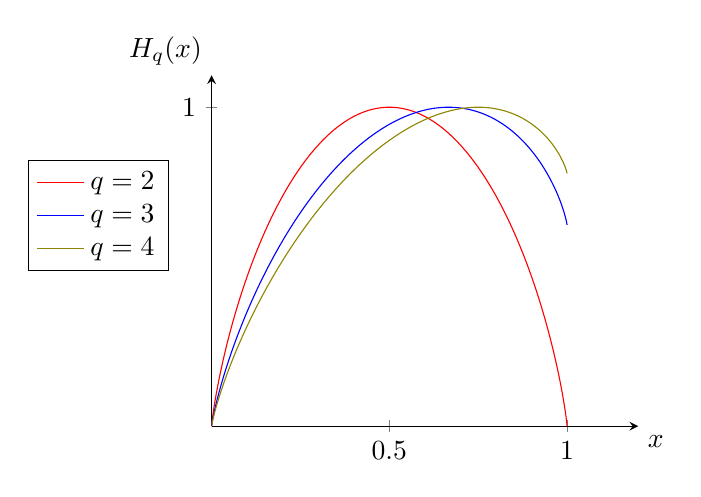
\begin{tikzpicture}
    \begin{axis}[
        xmin=0, xmax=1.2,
        ymin=0, ymax=1.1,
        xlabel=$x$, ylabel=$H_q(x)$,
        axis lines=middle,
        xtick={0.5,1},
        ytick={1},
        xlabel style={at={(ticklabel* cs:1)},anchor=north west},
        ylabel style={at={(ticklabel* cs:1)},anchor=south east},
        legend style={
            at={(-0.1,0.6)},
            anchor=east
            }
    ]
    \addplot[samples=1000, color=red, domain=0:1]{-x*log2(x)-(1-x)*log2(1-x)};
    \addplot[samples=1000, color=blue, domain=0:1]{x*ln(2)/ln(3)-x*ln(x)/ln(3)-(1-x)*ln(1-x)/ln(3)};
    \addplot[samples=1000, color=olive, domain=0:1]{x*ln(3)/ln(4)-x*ln(x)/ln(4)-(1-x)*ln(1-x)/ln(4)};
    
    \legend{$q=2$, $q=3$, $q=4$}
    \end{axis}
\end{tikzpicture}
\end{center}

$H_q$ attains its maximum value of $1$ at $1-\dfrac{1}{q}$.

\vspace{1mm}
The binary entropy function $H_2$ is denoted as $H_\mathsf{Ber}$.

\vspace{1mm}
Note that $$q^{-H_q(p)}=\left(\frac{p}{q-1}\right)^{p}(1-p)^{1-p}$$


\clearpage
\section{Introduction}

\subsection{Why is Coding Theory required?}
The English language has an enormous amount of redundancy. For instance, it's likely that the reader has seen the following text or something like it:

\vspace{1mm}
\texttt{Fi yuo cna raed tihs yuo hvae a sgtrane mnid. Olny srmat poelpe cna raed tish.}

\vspace{1mm}
While we have no doubt about the smartness of the reader, the above is \textit{not} a good test of the same. It merely means that the massive amount of redundancy in the language allows effective communication even in the presence of (an acceptable amount of) errors.

Of course, even in the digital realm, we expect to see errors as no system is truly foolproof. To understand the data even in the presence of errors, digital systems use redundancy as well.

\vspace{2mm}
Error-correcting codes (or just codes) are clever ways of representing data by introducing some redundancy such that the original data we want transmitted can be recovered even if parts of the data have errors.

When packets are transmitted over the internet, some packets get corrupted or lost in transmission. To deal with data corruption, a form of correction called ``CRC Checksum" is used. This is not a very good code. It searches for errors, and if an error is detected, it requests the data again. However, for obvious reasons, this is not always feasible. For instance, if we are receiving a transmission from a Mars Rover, we cannot just request the information again, it is simply not practical. Codes can also be seen in non-communication examples such as bank balances, bar codes and the memory of a computer. In these cases as well`, the data cannot be requested again.

\vspace{2mm}
In this report, we shall mainly focus on codes in the communication scenario. There is a sender who wants to send symbols over a noisy channel. He first encodes the symbols into a \textit{codeword} of $n$ symbols and sends it over the \textit{channel}. The receiver gets a \textit{received word} of $n$ symbols. He then tries to \textit{decode} the received word to recover the original symbols.

\vspace{2mm}
We make the assumption in this text that the sender and receiver have no method to communicate outside of the channel.

\vspace{2mm}
As we mentioned earlier, redundancy enables us to detect errors in a code with higher likelihood. A basic question that comes to mind is ``What is the minimum amount of redundancy required to ensure a high probability of detecting all errors in a code?"

\vspace{2mm}
The following diagram shows essentially what occurs in the process of encoding and decoding.

\begin{center}
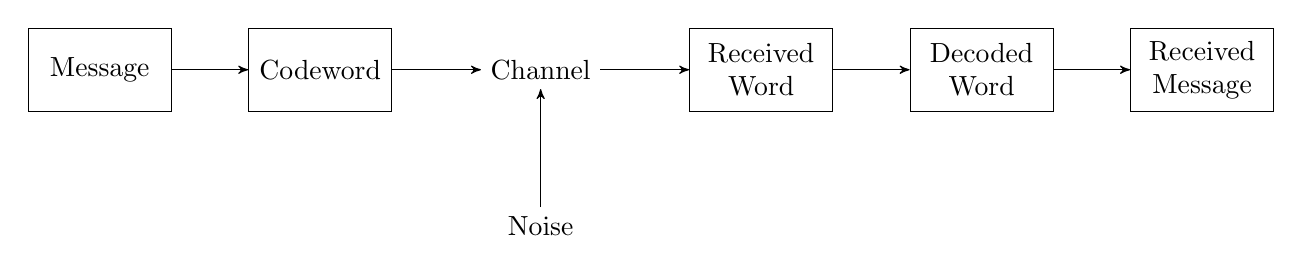
\begin{tikzpicture}[->, >=stealth', node distance=2.8cm, block_center/.style ={rectangle, draw=black, fill=white,
      text width=4.5em, text centered,
      minimum height=3em}]
    \node[block_center] (msg) {Message};
    \node[right of=msg, block_center] (codeword) {Codeword};
    \node[right of=codeword] (channel) {Channel};
    \node[right of=channel, align=center, block_center] (received) {Received\\Word};
    \node[right of=received, align=center, block_center] (decoded) {Decoded\\Word};
    \node[right of=decoded, align=center, block_center] (received2) {Received\\Message};
    \node[below=1.5cm of channel] (noise) {Noise};
    \draw (msg) edge (codeword)
          (codeword) edge (channel)
          (channel) edge (received)
          (received) edge (decoded)
          (decoded) edge (received2)
          (noise) edge (channel);
\end{tikzpicture}
\end{center}

During the course of this report, we primarily follow the texts \textit{A First Course in Coding Theory} \cite{hill} for sections $4$ through $6$ and \textit{Essential Coding Theory} \cite{esse} for sections $7$ through $9$.

\subsection{Basics and Definitions}

\begin{definition}
    A \textit{block code} $C$ over an alphabet $\Sigma$ is a non-empty subset of $\Sigma^n$ for some $n\in\mathbb{N}$.
\end{definition}

Henceforth, we shall refer to ``block code" as just ``code".

A \textit{$q$-ary code of length $n$} is a subset of $\Sigma^n$ where $|\Sigma|=q$.

\begin{definition}
    Elements of a code are called \textit{codewords}. The \textit{length} of a code $C$ over an alphabet $\Sigma$ is the $n$ for which $C\subseteq\Sigma^n$.
\end{definition}

A code $C$ of cardinality $M$ and length $n$ can be written as an $M\times n$ array whose rows are the codewords of $C$.

\begin{definition}
\label{dimCodeDef}
    Let $C$ be a code of cardinality $M$ over $\Sigma$ where $|\Sigma|=q$. Then the \textit{dimension} of $C$ is given by
    $$k=\log_q(M)$$
\end{definition}

\begin{example}
\label{parityCodeAndRepCodeExample}
    Let us look at two codes over $\mathbb{F}_2=\{0,1\}$. The first code is called the \textit{parity code}, denoted $C_\oplus$. Given any $(x_1,x_2,x_3)\in \{0,1\}^3$, its corresponding codeword is
    $$C_\oplus((x_1,x_2,x_3))=(x_1,x_2,x_3,x_1+x_2+x_3).$$
    That is, the final bit gives the sum of the first three bits modulo $2$. If a single error (a single bit-flip) occurs in $C_\oplus$, we can \textit{detect} it, since then the sum of the first three bits modulo $2$ will not be equal to the final bit.
    
    The second, called the \textit{repetition code} (represented $C_{n,\text{rep}}$), which is a very na\"ive approach involves repeating each bit $n$ times. For instance, for $n=3$, we have
    $$C_{3,\text{rep}}((x_1,x_2,x_3))=(x_1,x_1,x_1,x_2,x_2,x_2,x_3,x_3,x_3)$$
\end{example}


$C_{3,\text{rep}}$ is stronger since if a bit-flip occurs, not only can we detect it, we can \textit{correct} it and recover the original message by taking the symbol repeated $2$ or more times in each set of $3$ bits.

\vspace{2mm}
We shall now attempt to formalize the meanings of encoding and decoding. As we wish to send a message through a channel by converting it to a codeword and then sending the codeword, we may use $[|C|]$ to list all the messages that we can send.

\begin{definition}
    Let $C\subseteq\Sigma^n$. An equivalent description of the code $C$ is an injective mapping $E:[|C|]\to\Sigma^n$ called the \textit{encoding function}.
\end{definition}
 
To decode on the other hand, we must obtain a message from whatever word we receive (which may have errors).
 
\begin{definition}
    Let $C\subseteq\Sigma^n$ be a code. A mapping $D:\Sigma^n\to[|C|]$ is called a \textit{decoding function} of $C$.
\end{definition}


\begin{definition}
    For $\textbf{x}=(x_1,x_2,\ldots,x_n), \textbf{y}=(y_1,y_2,\ldots,y_n)\in\Sigma^n$, we define the \textit{Hamming distance} between $\textbf{x}$ and $\textbf{y}$ as
    $$d(\textbf{x},\textbf{y})=|\{i\in[n]\mid x_i\neq y_i\}|.$$
    If $\Sigma$ is a field, then for $\textbf{x}\in\Sigma^n$, we define the \textit{Hamming weight} of $\textbf{x}$ to be
    $$\wt(\textbf{x})=d(\textbf{x},\textbf{0})$$
    where $\textbf{0}$ represents the all zero vector $(0,0,\ldots,0)$.
\end{definition}

We see that the Hamming distance $d$ defines a metric on $\Sigma^n$ as
\begin{enumerate}
    \item $d(\textbf{x},\textbf{y})=0$ if and only if $\{i\in[n]\mid x_i\neq y_i\}=\emptyset$. This is equivalent to saying that $x_i=y_i$ for all $i\in[n]$, that is, $\textbf{x}=\textbf{y}$.
    \item $d(\textbf{x},\textbf{y})=|\{i\in[n]\mid x_i\neq y_i\}|=|\{i\in[n]\mid y_i\neq x_i\}|=d(\textbf{y},\textbf{x}).$
    \item Note that the minimum number of steps required to change $\textbf{x}$ to $\textbf{z}$ is $d(\textbf{x},\textbf{z})$. We can change $\textbf{x}$ to $\textbf{z}$ by changing $\textbf{x}$ to $\textbf{y}$ in $d(\textbf{x},\textbf{y})$ steps then $\textbf{y}$ to $\textbf{z}$ in $d(\textbf{y},\textbf{z})$ steps. This gives $d(\textbf{x},\textbf{z})\leq d(\textbf{x},\textbf{y})+d(\textbf{y},\textbf{z})$.
\end{enumerate}

Although the Hamming distance metric may not always be a very appropriate metric, it provides a good way to measure how ``close" two strings are.

\vspace{2mm}
We assume the following noise model called the \textit{Adversarial Noise Model}, which was first studied by Hamming:

\textit{Any error pattern can occur during transmission as long as the total number of errors is bounded. This means that both the location and the nature of the errors is arbitrary.}

\vspace{2mm}
We define error correction and detection in terms of the (Hamming) distance between a codeword and the word that is received after passing the codeword through the channel. Note that the output word is not fixed for a given codeword since we assume the Adversarial Noise Model.
\begin{definition}
    Let $C\subseteq\Sigma^n$ and let $t\geq 1$ be an integer. $C$ is said to be \textit{$t$-error correcting} if there exists a decoding function $D$ such that for every $\textbf{m}\in[|C|]$, $\textbf{y}\in\Sigma^n$ where
    \begin{enumerate}[(i)]
        \item $d(C(\textbf{m}),\textbf{y})\leq t$ and
        \item $C(\textbf{m})$ can become $\textbf{y}$ after passing through the channel,
    \end{enumerate}
    we have $D(\textbf{y})=\textbf{m}$.
\end{definition}

\begin{definition}
    Let $C\subseteq\Sigma^n$ and let $t\geq 1$ be an integer. $C$ is said to be \textit{$t$-error detecting} if there exists a detecting procedure $D:\Sigma^n\to\{0,1\}$ such that for every $\textbf{m}\in[|C|]$, $\textbf{y}\in\Sigma^n$ where
    \begin{enumerate}
        \item $1\leq d(C(\textbf{m}),\textbf{y})\leq t$ and
        \item $C(\textbf{m})$ can become $\textbf{y}$ after passing through the channel,
    \end{enumerate}
    we have $D(\textbf{y})=1$ if $\textbf{y}\in C$ and $0$ otherwise.
\end{definition}

So going back to the example discussed, $C_\oplus$ is a $1$-error detecting code and $C_{3,\text{rep}}$ is a $1$-error correcting code (and a $2$-error detecting code).

\begin{definition}
    If we receive a word $\textbf{y}$ after passing a codeword through a channel, \textit{nearest neighbour decoding} or \textit{minimum distance decoding} decodes $\textbf{y}$ as codeword $\textbf{x}'$ such that $d(\textbf{x}',\textbf{y})$ is minimum.
\end{definition}

\begin{definition}
    If we receive a word $\textbf{y}$ after passing a codeword through a channel, \textit{maximum likelihood decoding} decodes $\textbf{y}$ as codeword $\textbf{x}'$ such that $\Pr(\textbf{y}\text{ received}\mid \textbf{x}\text{ sent})$ is maximum.
\end{definition}

\vspace{2mm}
We now consider a specific type of channel.

\begin{definition}
    Consider an alphabet $\Sigma$. A corresponding channel is called a 
    \textit{$q$-ary symmetric channel} if
    \begin{enumerate}[(i)]
        \item Each symbol has the same probability $p<\frac{1}{2}$, called the \textit{symbol error probability}, of becoming erroneous.
        \item If a symbol becomes erroneous, then each of the $q-1$ other symbols of $\Sigma$ is equally likely to replace it.
    \end{enumerate}
\end{definition}

A $q$-ary symmetric channel is denoted $q\SC_p$ and a binary symmetric channel is denoted $\BSC_p$.

Note that if the error vector $\textbf{e}$ is drawn from $q\mathsf{SC}_p$, $\wt(\textbf{e})$ follows a binomial distribution with parameters $n$ and $p$.

\vspace{2mm}
The probability that a received codeword of length $n$ has an error in exactly $i$ specific places is $p^{i}(1-p)^{n-i}$. Since $p<\frac{1}{2}$, it is more probable that a fewer number of errors occur.

\vspace{2mm}
Consider the code $C=\{000,111\}$ for the binary alphabet $\{0,1\}$ passed through a binary symmetric channel. Say $000$ is transmitted. Then following nearest neighbour decoding, the probability that the received codeword is decoded as $000$ (that is, the received codeword is $000,100,010$ or $001$) is $(1-p)^3+3p(1-p)^2=(1-p)^2(1+2p)$. For any word $\textbf{c}$ in $C$, the \textit{word error probability} of $C$, denoted $P_\text{err}(\textbf{c})$, denotes the probability that $\textbf{c}$ is interpreted incorrectly after passing through a channel (Note that by symmetry, this is equal for any codeword in this case). Here,
$$P_\text{err}(\textbf{c})=1-(1-p)^2(1+2p)=3p^2-2p^3.$$

\begin{definition}
    For any code $C$, the \textit{minimum distance} is defined as
    $$d(C)=\min\{d(\textbf{x},\textbf{y})\mid \textbf{x},\textbf{y}\in C, \textbf{x}\neq \textbf{y}\}.$$
\end{definition}

\begin{theorem}
\label{DetectAndCorrectForGivenMinDist}
\phantom{owo}
\begin{enumerate}[(i)]
    \item A code $C$ is $s$-error detecting if $d(C)>s$.
    \item A code $C$ is $s$-error correcting $d(C)>2s$.
\end{enumerate}
\end{theorem}
\begin{proof}
\phantom{uwu}
\begin{enumerate}[(i)]
    \item Suppose a codeword $\textbf{x}$ is transmitted, and the received codeword $\textbf{y}$ has $s$ or fewer errors. Then $d(\textbf{x},\textbf{y})\leq s$ and as $\textbf{x}\in C$, $\textbf{y}\not\in C$ and the error can be detected.
    \item Supposed a codeword $\textbf{x}$ is transmitted and the received codeword $\textbf{y}$ has $s$ or fewer errors. Then $d(\textbf{x},\textbf{y})\leq s$. We claim that the codeword $\textbf{x}'$ such that $d(\textbf{x}',\textbf{y})$ is minimum is unique and equal to $\textbf{x}$. If $\textbf{x}'\neq \textbf{x}$, then $d(\textbf{y},\textbf{x}')\leq d(\textbf{x},\textbf{y})\leq s$. Then $d(\textbf{x},\textbf{x}')\leq d(\textbf{x},\textbf{y})+d(\textbf{y},\textbf{x}')\leq s+s=2s$ as $d$ is a metric. However, we have $d(C)>2s$, which is a contradiction. Thus, $\textbf{x}'=\textbf{x}$ and $C$ can correct up to $s$ errors.
\end{enumerate}
\end{proof}

\begin{corollary}
    Let a code $C$ have minimum distance $d$. Then
    \begin{enumerate}[(i)]
        \item $C$ is $(d-1)$-error detecting.
        \item $C$ is $\left\lfloor{\dfrac{d-1}{2}}\right\rfloor$-error correcting.
    \end{enumerate}
\end{corollary}
\begin{proof}
    We have $d>s$ if and only if $s\leq d-1$ and $d>2s$ if and only if $s\leq \left\lfloor\dfrac{d-1}{2}\right\rfloor$. Combining this with \ref{DetectAndCorrectForGivenMinDist} gives the required result.
\end{proof}

\textit{Notation.} An \textit{$(n,M,d)_q$-code} is a code of length $n$, cardinality $M$ and minimum distance $d$ over an alphabet $\Sigma$ such that $|\Sigma|=q$.

For example, the code $\{000,111\}$ over $\{0,1\}$ is a $(3,2,3)_2$-code.

\begin{definition}
    Let $C$ be a code of length $n$ and minimum distance $d$. The \textit{relative distance} of $C$ is given by
    $\delta=\frac{d}{n}.$
\end{definition}

\begin{definition}
    For $q,n\in\mathbb{N}$, the \textit{repetition code of length $n$} over an alphabet $\Sigma$ is the code whose codewords are $aa\cdots a$ (repeated $n$ times) where $a\in\Sigma$.
\end{definition}

A $q$-ary repetition code of length $n$ is an $(n,q,n)_q$-code. It is represented by $C_{n,\text{rep}}$.

\clearpage
\section{Bounds on the Number of Codewords}

An ideal $(n,M,d)_q$-code has a small value of $n$ (so the data can be transmitted faster), a large value of $M$ (so a larger number of messages can be transmitted), and a large value of $d$ (to detect/correct many errors).

\subsection{Some Useful Bounds}

We shall attempt to optimize the value of $M$ keeping the other two fixed.

\begin{definition}
We denote by $A_q(n,d)$ the largest value of $M$ such that there exists a $q$-ary $(n,M,d)_q$-code.
\end{definition}

\begin{theorem}
For all $n,q\in\mathbb{N}$,
\begin{enumerate}[(i)]
    \item $A_q(n,1)=q^n$.
    \item $A_q(n,n)=q$.
\end{enumerate}
\end{theorem}
\begin{proof}
\phantom{owo}
\begin{enumerate}[(i)]
    \item $M\leq q^n$ as the code is a subset of $\Sigma^n$. As $\Sigma^n$ is of length $n$ and has minimum distance $1$, $A_q(n,1)=q^n$.
    \item If the minimum distance of a code is $n$, any two codewords differ at all $n$ places. Thus the symbols appearing in any fixed position in the $M$ codewords must be distinct, giving $M\leq q$. The $q$-ary repetition code of length $n$ is an $(n,q,n)_q$-code so $A_q(n,n)=q$.
\end{enumerate}
\end{proof}

\begin{definition}
\label{equivalent1}
    Two $q$-ary codes are \textit{equivalent} if one can be obtained from the other by a combination of the following operations:
    \begin{enumerate}[(i)]
        \item permutation of the positions of the code.
        \item permutation of the symbols appearing in a fixed position.
    \end{enumerate}
\end{definition}

Note that if we represent an $(n,M,d)_q$-code as an $M\times n$ array, (i) corresponds to rearranging the columns and (ii) corresponds to a renaming of the symbols in a given column.

As distances between codewords remain the same, two equivalent codes have the same value of length, cardinality, and minimum distance.

\begin{lemma}
    Any $(n,M,d)_q$-code over $\{0,1,\ldots,q-1\}$ is equivalent to an $(n,M,d)_q$-code (over $\{0,1,\ldots,q-1\}$) that contains the codeword $\textbf{0}=000\cdots 0$.
\end{lemma}
\begin{proof}
    Consider any codeword $x=x_1x_2\cdots x_n$. For each $i$, apply the permutation of symbols
    $$\left(\begin{matrix}x_i & 0 & j & \\ \downarrow & \downarrow & \downarrow & \text{for all $j\neq x_i,0$} \\ 0 & x_i & j & \end{matrix}\right).$$
\end{proof}

Let $\Sigma=\mathbb{F}_2$. For some $n\in\mathbb{N}$, consider $x,y$ be two vectors in $\Sigma^n$, where $x=x_1x_2\cdots x_n$ and $y=y_1y_2\cdots y_n$. $x+y$ is given by the component wise sum in $\mathbb{F}_2$. $x\cap y$ is defined to be the component wise multiplication in $\mathbb{F}_2$. That is, $x+y=(x_1+y_1, x_2+y_2, \ldots, x_n+y_n)$ and $x\cap y=(x_1y_1, x_2y_2,\ldots, x_ny_n)$.
    
\begin{lemma}
    For any $x,y\in\mathbb{F}_2^n$, $d(x,y)=\wt(x+y)$.
\end{lemma}
\begin{proof}
    $x+y$ has a $1$ wherever $x_i\neq y_i$ and $0$ elsewhere. As $\wt(x)$ is just the number of $1$s in $x$, $d(x,y)=\wt(x+y)$.
\end{proof}

\begin{lemma}
\label{BinaryDistancePIE}
    For any $x,y\in\mathbb{F}_2^n$, $d(x,y)=\wt(x)+\wt(y)-2\wt(x\cap y)$.
\end{lemma}
\begin{proof}
    We have $d(x,y)=\wt(x+y)$, the number of $1$s in $x+y$, from the previous lemma. This is given by the number of positions with $1$ in $x$ $+$ the number of positions with $1$ in $y$ $-$ the number of positions with $1$ in both $x$ and $y$. This is just $\wt(x)+\wt(y)-2\wt(x\cap y)$.
\end{proof}

\begin{theorem}
    Let $d$ be odd. Then a binary $(n,M,d)_2$-code exists if and only if a binary $(n+1,M,d+1)_2$-code exists.
\end{theorem}
\begin{proof}
    Let $C$ be a binary $(n,M,d)_2$-code for odd $d$. Construct a code $C'$ such that for each $x=x_1x_2\cdots x_n\in C$, we extend it to $x'=x_1x_2\cdots x_{n+1}$ where $x_{n+1}=\sum_{i=1}^n x_i$. This is called adding an \textit{overall parity check}.
    
    \vspace{1mm}
    As $\wt(x')$ is even for any $x'\in C'$ (because $\wt(x')\equiv 2x_{n+1}\Mod 2$), $d(C')$ is even by \ref{BinaryDistancePIE}. Clearly, $d\leq d(C')\leq d+1$. As $d$ is odd, $d(C')=d+1$. Thus $C'$ is an $(n+1,M,d+1)_2$ code.
    
    \vspace{2mm}
    In the other direction, let $C'$ be a binary $(n+1,M,d+1)_2$-code. Choose $x,y\in C'$ such that $d(x,y)=d+1$. Construct a code by choosing any position where they differ and deleting this position from all codewords. The resulting code has minimum distance $d$ and is thus an $(n,M,d)_2$-code.
\end{proof}

\begin{corollary}
    Let $d$ be odd. then $A_2(n+1,d+1)=A_2(n,d)$.
\end{corollary}
\begin{proof}
    This follows from the previous theorem.
\end{proof}

\begin{definition}
    For any $u\in\Sigma^n$ (where $|\Sigma|=q$) and any integer $r\geq 0$, the \textit{Hamming ball} or \textit{sphere} of radius $r$ and centre $u$ is given by
    $$B_q(u,r)=\{v\in\Sigma^n\mid d(u,v)\leq r\}.$$
\end{definition}

If $q$ is understood, we simply write $B(u,r)$.

\vspace{2mm}
This gives more insight into why a code is $s$-error correcting if $d(C)>2s$ (if $u$ is received, the transmitted codeword will be the unique codeword in $B_q(u,s)$).

\begin{lemma}
\label{numWordsInSphere}
    Let $\Sigma$ contain $q$ symbols. The number of words in a ball of radius $r$ in $\Sigma^n$ is exactly
    $$\sum_{i=0}^r \binom{n}{i}(q-1)^i.$$
\end{lemma}
\begin{proof}
    The number of words at a distance of exactly $i$ from a given word $x$ is given by choosing exactly $i$ positions from the $n$ positions and then picking one of $q-1$ symbols to replace the symbol at each of those positions. This is equal to $\binom{n}{i}(q-1)^i$. The required result is the sum of this quantity over $\{i:0\leq i\leq r\}$.
\end{proof}

\begin{theorem}[The Hamming bound]
\label{hammingBound}
    An $(n,M,2t+1)_q$-code satisfies
    $$M\sum_{i=0}^t \binom{n}{i}(q-1)^i\leq q^n.$$
\end{theorem}
\begin{proof}
    Note that two balls of radius $t$ centered at distinct codewords have no words in common as the minimum distance of the code is $2t+1$. The number of words in each ball is $\sum_{i=0}^t\binom{n}{i}(q-1)^i$ by \ref{numWordsInSphere}. The total number of words in the $M$ balls is $M$  multiplied by this quantity, which must be less than or equal to $q^n$, the total number of words in $\Sigma^n$. This gives the required result.
\end{proof}

The Hamming bound provides an upper bound on $A_q(n,d)$.

In general for an $(n,M,d)_q$-code, 
$$M\sum_{i=0}^{\left\lfloor\frac{d-1}{2}\right\rfloor} \binom{n}{i}(q-1)^i\leq q^n.$$

In the binary case, the Hamming bound gives
$$M\sum_{i=0}^{\left\lfloor\frac{d-1}{2}\right\rfloor}\binom{n}{i}\leq 2^n.$$

For an $(n,M,d)_q$-code of dimension $k$,
$$k\leq n - \log_q\left(\sum_{i=0}^{\left\lfloor\frac{d-1}{2}\right\rfloor} \binom{n}{i}(q-1)^i\right)$$

% However, the Hamming bound is not particularly useful in binary codes when $n<2d$. 

\subsection{Perfect Codes}

A code which achieves the Hamming bound is called a \textit{perfect code}.

\begin{definition}
    An $(n,M,d)_q$-code is called a \textit{perfect code} if it satisfies
    $$M\sum_{i=0}^{\left\lfloor\frac{d-1}{2}\right\rfloor} \binom{n}{i}(q-1)^i = q^n.$$
\end{definition}

The repetition code of length $n$, where $n$ is odd, is a perfect code. These codes, along with codes that contain exactly one codeword and codes that are the entirety of $\Sigma^n$, are called \textit{trivial} perfect codes.

\vspace{2mm}
An example of a nontrivial perfect code is the following.

Let $\textbf{0}=0000000$, $\textbf{1}=1111111$, $a_1=1101000$, $a_2=0110100$, $a_3=0011010$, $a_4=0001101$, $a_5=1000110$, $a_6=0100011$, $a_7=1010001$. We further define $b_i$ as the same as $a_i$ except that all $0$s are replaced with $1$s and all $1$s are replaced with $0$s. Then the code $C$ containing $\textbf{0}, \textbf{1}$, all the $a_i$s and all the $b_i$s is a (nontrivial) perfect code.
Note that the $a_i$s correspond to the rows of the matrix in \ref{incidenceMatrixOf77331Des}.

\vspace{2mm}
For any $i,j\in[7]$, $i\neq j$,
$$d(a_i,a_j)=\wt(a_i)+\wt(a_j)-2\wt(a_i+a_j)=3+3-2=4.$$
Also, $d(\textbf{0}, a_i)=d(\textbf{1}, b_i)=3$ and $d(\textbf{0}, b_i)=d(\textbf{1}, a_i)=4$.

Finally, $a_i$ and $b_j$ differ exactly where $a_i$ and $a_j$ agree so $d(a_i,b_j)=7-d(a_i,a_j)=3$.

Thus $C$ is a $(7,16,3)_2$-code. It may be checked that this is a perfect code.

\vspace{2mm}
We shall study perfect codes more in detail later on.

\begin{theorem}
    If there exists a Hadamard $(4t-1,2t-1,t-1)$-design, then
    $$A_q(4t-1,2t-1)\geq 8t.$$
\end{theorem}
\begin{proof}
    Similar to the construction described above, construct a code $C$ containing $\textbf{0}$, $\textbf{1}$, the vectors $a_i$ corresponding to each of the rows of the incidence matrix of the Hadamard design and the vectors $b_i$ which are the same as $a_i$ except that all $0$s are replaced with $1$s and all $1$s are replaced with $0$s.
    
    \vspace{1mm}
    As each vertex is present in exactly $2t-1$ blocks, there are $(2t-1)$ $1$s in each row and thus
    $$d(\textbf{0}, a_i)=2t-1 \text{ for all valid $i$.}$$
    Similarly,
    $$d(\textbf{0}, b_i)=d(\textbf{1}, a_i)=2t\text{ and } d(\textbf{1}, b_i)=2t-1.$$
    We also have 
    \begin{align*}
        d(a_i,a_j) &= \wt(a_i)+\wt(a_j)-2\wt(a_i\cap a_j) \\
                   &= 2t-1+2t-1-2\wt(a_i\cap a_j).    
    \end{align*}
    
    As mentioned earlier, $\wt(a_i)=\wt(a_j)=2t-1$. $\wt(a_i\cap a_j)$ is the number of blocks in which the vertices corresponding to $a_i$ and $a_j$ are both present, which is equal to $t-1$.
    
    Thus, $d(a_i, a_j)=(2t-1)+(2t-1)-2(t-1)=2t-1$ for all valid $i,j$. Similarly, we get $d(b_i,b_j)=2t-1$ and $d(a_i, b_j)=2t$.
    
    \vspace{1mm}
    The number of codewords in this code is $2+2(4t-1)=8t$. The minimum distance of this code is $2t-1$ and its length is $4t-1$.
    
    Therefore, the resulting code is a $(4t-1,8t,2t-1)_2$-code.
\end{proof}

This provides another bound on $A_q(n,d)$. Namely, if a Hadamard $(4t-1,2t-1,t-1)$-design exists, $A_q(4t-1,2t-1)\geq 8t$.

\clearpage
\section{Linear Codes}

\subsection{Introduction to Linear Codes}

\begin{definition}
    A \textit{linear code} over $\mathbb{F}_q$ is a subspace of $V(n,q)$ for some positive integer $n$.
\end{definition}

Note that the dimension (recall \ref{dimCodeDef}) of a linear code is equal to its dimension as a vector space.

We denote by $\textbf{0}$ the element of a linear code that consists of all $0$s.

If a linear code is a $k$-dimensional subspace of $V(n,q)$, we call it an $[n,k]_q$-code. If we further wish to specify the minimum distance $d$ of the code, we call it an $[n,k,d]_q$-code.

\begin{lemma}
    If $x,y\in V(n,q)$, then $d(x,y)=\wt(x-y)$.
\end{lemma}
\begin{proof}
    $x-y$ is nonzero exactly wherever $x$ and $y$ differ. The result follows.
\end{proof}

\begin{theorem}
\label{minDistIsMinWeight}
    Let $C$ be a linear code and $\wt(C)=\min\{\wt(x)\mid x\in C\setminus\{0\}\}$. Then $d(C)=\wt(C)$.
\end{theorem}
\begin{proof}
    There exist $x,y\in C$ such that $d(x,y)=d(C)$, that is, $\wt(x-y)=d(C)$. This gives $d(C)=\wt(x-y)\geq \wt(C)$ since $x-y\in C$.
    
    Let $x\in C$ such that $\wt(x)=\wt(C)$. Then $\wt(C)=d(x,\textbf{0})\geq d(C)$.
    
    This gives $d(C)=\wt(C)$.
\end{proof}

Note that to find the minimum distance in any general code, we must make $\binom{m}{2}$ comparisons, but in a linear code, we only need to examine the weights of $M-1$ codewords.

% \begin{theorem}
%     In a binary linear code $C$, either all the codewords have even weight or exactly half have even weight and half have odd weight.
% \end{theorem}
% \begin{proof}
%     Let $w\in C$ have odd weight. If no such $x$ exists, then all codewords have even weight. Let $C_e$ be the subset of $C$ which contains all codewords of even weight and $C_o$ the subset of $C$ which contains all codewords of odd weight.
    
%     Consider the function $f:C_e\to C_o$ defined by $x\mapsto x+w$ for $x\in C_e$. This function makes sense as given any $x\in C_e$, $\wt(x+w)=\wt(x)+\wt(w)-2\wt(x\cap w)$. As $\wt(x)+\wt(w)$ is odd, $x+w\in C_o$. We claim that $f$ is a bijection. Given any $y\in C_o$, $y-w\in C_e$ by a similar argument that we used to show that that the function is well-defined. This shows that the map is surjective. Next, given any $x,y\in C_e$, $x+w=y+w\implies x=y$ so the map is injective and thus bijective. Thus, $|C_e|=|C_o|$ if $C_o$ is non-empty. The result follows.
% \end{proof}

\begin{definition}
    Let $C$ be an $[n,k]_q$-code. A $k\times n$ matrix whose rows form a basis of $C$ is called a \textit{generator matrix} of $C$.
\end{definition}

Note that if $G$ is a generator matrix of an $[n,k]_q$-code $C$, $C=\{\textbf{x}G\mid \textbf{x}\in V(n,k)\}$.

For example, the generator matrix of the $q$-ary repetition code of length $n$ over $\mathbb{F}_q$ is the $1\times n$ matrix $\begin{pmatrix}1 & 1 & \cdots & 1\end{pmatrix}$.

\begin{definition}
    Two linear codes over $\mathbb{F}_q$ are called \textit{equivalent} if one can be obtained from the other by a combination of the following operations:
    \begin{enumerate}[(i)]
        \item Permutation of the positions of the code.
        \item Multiplication of the symbols appearing in a fixed position by a non-zero scalar.
    \end{enumerate}
\end{definition}

Alternatively, two linear codes are equivalent if they are isomorphic.

Note that this is \textit{not} the same as the definition of equivalence we gave earlier in \ref{equivalent1}.

\begin{theorem}
    Two $k\times n$ matrices generate the same $[n,k]_q$-code over $\mathbb{F}_q$ if one matrix can be obtained from the other by a combination of the following operations:
    \begin{enumerate}[(i)]
        \item Permutation of the rows.
        \item Multiplication of a row by a non-zero scalar.
        \item Addition of scalar multiple of one row to another.
        \item Permutation of the columns.
        \item Multiplication of a column by a non-zero scalar.
    \end{enumerate}
\end{theorem}
\begin{proof}
    The first three conditions merely replace one basis of the code with another. The final two conditions are those in the definition of equivalence of linear codes.
\end{proof}

\begin{theorem}
    Let $G$ be a generator matrix of an $[n,k]_q$-code. $G$ generates the same code as as a matrix in the \textit{standard form} $(I_k\mid A)$, where $I_k$ is the $k\times k$ identity matrix and $A$ is a $k\times (n-k)$ matrix.
\end{theorem}
\begin{proof}
    Let $G=(g_{ij})$ and let $\textbf{r}_1,\textbf{r}_2,\ldots,\textbf{r}_k$ and $\textbf{c}_1,\textbf{c}_2,\ldots,\textbf{c}_n$ be the rows and columns of the matrix respectively. We repeat the following three step procedure for $j=1,2,\ldots,k$, which transforms $\textbf{c}_j$ into the required form leaving the first $j-1$ columns unchanged. Suppose that $G$ has already been transformed to
    $$
    \begin{pmatrix}
    1 & 0 & \cdots & 0 & g_{1j} & \cdots & g_{1n} \\
    0 & 1 & \cdots & 0 & g_{2j} & \cdots & g_{2n} \\
    \vdots & \vdots &  & \vdots & \vdots & & \vdots \\
    0 & 0 & \cdots & 1 & g_{j-1,j} & \cdots & g_{j-1,n} \\
    0 & 0 & \cdots & 0 & g_{jj} & \cdots & g_{jn} \\
    \vdots & \vdots & & \vdots & \vdots & & \vdots \\
    0 & 0 & \cdots & 0 & g_{nj} & \cdots & g_{nn}
    \end{pmatrix}.
    $$
    \begin{enumerate}
        \item if $g_{jj}=0$ and $g_{ij}\neq 0$ for some $i>j$, we interchange $\textbf{r}_i$ and $\textbf{r}_j$. Otherwise, if $g_{jj}=0$ and $g_{ji}\neq 0$ for some $i>j$, interchange $\textbf{c}_i$ and $\textbf{c}_j$ (the existence of such an $i$ is guaranteed by the fact that the rows are linearly independent).
        \item Multiply $\textbf{r}_j$ with $g_{jj}^{-1}$ (which is well-defined as $g_{jj}\neq 0$).
        \item For each $i=1,2,\ldots,k$, replace $\textbf{r}_i$ with $\textbf{r}_i-g_{ij}\textbf{r}_j$.
    \end{enumerate}
    The column $\textbf{c}_j$ then has the required form. After we repeat this procedure for $j=1,2,\ldots,k$, the generator matrix will be in standard form.
\end{proof}

\subsection{Encoding and Decoding with Linear Codes}

Let $C$ be an $[n,k]_q$-code with generator matrix $G$ over $\mathbb{F}_q$. For any $\textbf{u}\in V(k,q)$ (here we represent $\textbf{u}$ by a row vector), we have $\textbf{u}G\in C$ as this is merely a linear combination of the row vectors of $G$.

\vspace{2mm}
This suggests a way to encode message vectors of $\mathbb{F}_q^k$. Note that the encoding function briefly described above given by $\textbf{u}\mapsto \textbf{u}G$ for $\textbf{u}\in V(k,q)$ maps the vector space $V(k,q)$ onto $C$.

\vspace{2mm}
This is even easier to understand in the case where the generator matrix is in standard form. Let $G=(I_k\mid A)$ where $A=(a_{ij}i$ implies is a $k\times (n-k)$ matrix.
The message vector $\textbf{u}$ is encoded as $\textbf{x}=\textbf{u}G=x_1x_2\cdots x_kx_{k+1}\cdots x_n$. Here, $x_i=u_i$ for $1\leq i\leq k$ and $x_i=\sum_{j=1}^k a_{ji}u_j$ for $k+1\leq i\leq n$.

\vspace{1mm}
Note that in addition to the message $\textbf{u}$, $\textbf{x}$ contains extra information. The message digits $x_{k+1},x_{k+2},\ldots,x_n$ are called \textit{check digits} and represent the redundancy we mentioned at the start of this report. They provide protection against any errors that might occur.

\vspace{2mm}
Now, suppose the codeword $\textbf{x}$ is sent through the channel and the received codeword is $\textbf{y}$. We define the \textit{error vector} $\textbf{e}$ to be $$\textbf{e}=\textbf{y}-\textbf{x}.$$

\begin{definition}
    Suppose that $C$ is an $[n,k]_q$-code over $\mathbb{F}_q$ and $\textbf{a}\in V(n,q)$. Then for $\textbf{a}\in C$, the \textit{coset} $\textbf{a}+C$ is given by
    $$\textbf{a}+C=\{\textbf{a}+\textbf{x}\mid \textbf{x}\in C\}.$$
\end{definition}

This corresponds to \ref{cosetDef} considering $V(n,q)$ as a group under addition.

\begin{lemma}
    The set of cosets of a code in $V(n,q)$ partition $V(n,q)$. Furthermore, for $\textbf{a},\textbf{b}\in V(n,q)$, $\textbf{a}+C=\textbf{b}+C$ if and only if $\textbf{b}\in \textbf{a}+C$.
\end{lemma}
\begin{proof}
    This follows from \ref{cosetPartition}.
\end{proof}

\begin{theorem}[Lagrange's Theorem]
    Suppose $C$ is an $[n,k]_q$-code over $\mathbb{F}_q$. Then every coset of $C$ in $V(n,q)$ contains exactly $q^k$ elements.
\end{theorem}
\begin{proof}
    This follows from \ref{LagrangesTheorem}.
\end{proof}

\begin{definition}
    A vector having minimum weight in a coset is called a \textit{coset leader}. If a coset has more than one vector of minimum weight, we choose any such vector and call it the coset leader.
\end{definition}


A \textit{Slepian standard array} or simply \textit{standard array} of an $[n,k]_q$-code $C$ is a $q^{n-k}\times q^k$ array of the elements of $V(n,q)$ which is constructed as follows.
\begin{enumerate}
    \item List the codewords of $C$, starting with $\textbf{0}$, in the first row.
    \item Choose any vector of minimum weight not already in the array. Write this as the first entry of the following row. Denote this vector as the coset leader.
    \item Fill out the row by adding the coset leader to the codeword at the top of each column. The sum of the coset leader of row $i$ and the $j$th codeword becomes the $i,j$th element of the array.
    \item Repeat the above two steps until all the cosets and every vector of $V(n,q)$ appears in the array.
\end{enumerate}
That is, each row of the standard array represents a coset with the coset leader written on the left.

Note that any element of the array is equal to the sum of the first element of the row and column of said element.

For example, the standard array corresponding to the code $C=\{0000,1011,0101,1110\}$ is
\begin{center}
\begin{tabular}{|c|c|c|c|}
    \hline
     0000 & 1011 & 0101 & 1110 \\ \hline
     1000 & 0011 & 1101 & 0110 \\ \hline
     0100 & 1111 & 0001 & 1010 \\ \hline
     0010 & 1001 & 0111 & 1100 \\ \hline
\end{tabular}
\end{center}

\vspace{2mm}
Now, if we want to decode a received vector, we may do so by identifying the error vector $\textbf{e}$ with the first element of the row containing the received vector and the decoded word as the first element of the column. That is, we decode an element as the codeword at the top of its column in the standard array.

\vspace{1mm}
The error vectors which will be corrected are precisely the coset leaders.

\vspace{2mm}
Let $C$ be an $[n,k,2t+1]_q$-code. Then $C$ can correct any $t$ errors. This implies every vector of weight $i\leq t$ is a coset leader. Determining the number of coset leaders of weight $i>t$ is problematic in the general case however. It is easy to establish that in the case of perfect codes, this is equal to $0$ for each $i>t$. However, these values are not known even for several well-known families of codes.

\vspace{2mm}
The primary issues with standard array decoding are that
\begin{itemize}
    \item It requires a massive amount of storage as we store every single vector in $V(n,q)$. For example, a binary code of length $32$ would require $2^{32}$ entries.
    \item It takes a large amount of time to locate a given vector in the array due to its size.
\end{itemize}

\subsection{Some results on Binary Linear Codes}
We now restrict ourselves to binary linear codes. We assume that the channel is a binary symmetric channel with symbol error probability $p$.

\begin{theorem}
    Let $C$ be a binary $[n,k]_2$-code and for $i=0,1,\ldots,n$ let $\alpha_i$ denote the number of coset leaders of weight $i$. Then the probability that a decoded vector decoded using a standard array is the codeword $\textbf{c}$ which was sent is
    $$P_\text{corr}(\textbf{c})=\sum_{i=0}^n\alpha_ip^i(1-p)^{n-i}$$
\end{theorem}
\begin{proof}
    The probability that the error vector is a given vector of weight $i$ is $p^i(1-p)^{n-i}$. As there are $\alpha_i$ such errors, the probability that the error vector is one of the acceptable error vectors is the sum of $\alpha_ip^i(1-p)^{n-i}$ over $i=0,1,2,\ldots,n$.
\end{proof}

The probability that the decoded word is \textit{not} the codeword $\textbf{c}$ sent, called the \textit{word error rate}, is given by
$$P_\text{err}(\textbf{c})=1-P_\text{corr}(\textbf{c}).$$

\begin{definition}
    Let $C$ be an $[n,k]_q$-code. The \textit{rate} of $C$ is defined by $$R(C)=\frac{k}{n}.$$
\end{definition}

The rate captures a way to measure the redundancy of a code. The higher the redundancy, the lower the rate is. Therefore, an efficient code will have a high rate.

\vspace{2mm}
A natural question to ask would be:

\textit{Given a code of distance $d$, what is the largest rate $R$ that it can have?}

% \subsection{Symbol Error Rate}

% Oftentimes, a more useful quantity is the \textit{symbol error rate} $P_\text{symb}$, which is the average probability that a symbol is in error after decoding.

% \begin{theorem}
%     If a standard array is used for a binary $[n,k]_2$-code and the messages are equally likely, then $P_\text{symb}$ does not depend on which codeword was sent and is given by
%     $$P_\text{symb}=\frac{1}{k}\sum_{i=1}^{2^k}F_iP_i$$
%     where $F_i$ is the weight of the first $k$ places of the codeword at the top of the $i$th column of the standard array and $P_i$ is the probability that the error vector is in this $i$th column. 
% \end{theorem}
% \begin{proof}
%     Let $\textbf{u}=u_1u_2\cdots u_k\in V(k,2)$ be the initial message vector. $\textbf{u}$ is encoded to $x=x_1x_2\cdots x_n$ where $x_i=u_i$ for $1\leq i\leq k$. After passing through the channel, the received word is $\textbf{y}=y_1y_2\cdots y_n$. The decoded word is the vector at the top of the column of the standard array that contains $\textbf{y}$ and the received message is the first $k$ symbols of the decoded word.
    
%     The symbol error rate is merely the probability that $\textbf{y}$ is in a different column than $\textbf{x}$. The probability that $\textbf{y}$ is in the same column as $\textbf{x}$ is equal to the probability the error vector is one of the coset leaders.
% \end{proof}

% \begin{theorem}
%     For a binary $[n,k]_2$-code,
%     $$\frac{1}{k}P_\text{err}\leq P_\text{symb}\leq P_\text{err}.$$
% \end{theorem}

\subsection{Error Detection in  Binary Linear Codes}

We now consider error \textit{detection}. If the codeword sent is $\textbf{x}$, we will fail to detect an error if and only if the received vector $\textbf{y}$ is a codeword as well, that is, $\textbf{e}=\textbf{y}-\textbf{x}$ is a codeword.

For any code $C$ and $\textbf{c}\in C$, we denote by $P_\text{undetec}(\textbf{c})$ the probability that an incorrect codeword is received, which is independent of the codeword sent in the binary symmetric channel case.

\begin{theorem}
    Let $C$ be a binary $[n,k]_2$-code transmitted through a binary symmetric channel of symbol error probability $p$. Let $A_i$ be the number of codewords of $C$ of weight $i$ for each valid $i$. Then if $C$ is used for error detection, for any $\textbf{c}\in C$,
    $$P_\text{undetec}(\textbf{c})=\sum_{i=1}^n A_ip^i(1-p)^{n-i}.$$
\end{theorem}
\begin{proof}
    We must simply find the probability that the error vector is in $C$. As the probability that there are exactly $i$ specific errors is $p^i(1-p)^{n-i}$ and there are $A_i$ codewords of weight $i$, the result follows.
\end{proof}

If we detect an error, we might ask to retransmit the data again. In this case, the probability that we will request retransmission is given by
$$P_\text{retrans}(\textbf{c})=1-(1-p)^n-P_\text{undetec}(\textbf{c}).$$
The above follows as $(1-p)^n$ is the probability that no error occurs and $P_\text{undetec}$ is the probability that an error occurs but we do not detect it.

\subsection{The Dual Code}

\begin{definition}
    Let $C$ be a linear $[n,k]_q$-code. The \textit{dual code} of $C$, denoted $C^\perp$, is the orthogonal subspace of $C$ with respect to $V(n,q)$, that is,
    $$C^\perp=\{\textbf{v}\in V(n,q)\mid \textbf{v}\perp\textbf{w}\text{ for all }\textbf{w}\in C\}.$$
\end{definition}

\begin{lemma}
\label{perpIffvGT=O}
    Let $C$ be an $[n,k]_q$-code with generator matrix $G$. Then $\textbf{v}\in V(n,q)$ is an element of $C^\perp$ if and only if $\textbf{v}G^\text{T}=O$.
\end{lemma}
\begin{proof}
    Let $\textbf{r}_1,\textbf{r}_2,\ldots,\textbf{r}_k$ be the row vectors of $G$ which form a basis of $C$.
    
    If $\textbf{v}\in C^\perp$, then $\textbf{v}$ is orthogonal to every element of $C$ and in particular, the row vectors of $G^\text{T}$, so the `only if' part of the lemma follows.
    
    To prove the `if' part of the lemma, let $\textbf{u}$ be any element of $C$. We have that $\textbf{v}\cdot\textbf{r}_i$ for each $i$ as $\textbf{v}G^\text{T}=0$. Then $u=a_1\textbf{r}_1+a_2\textbf{r}_2+\cdots+a_k\textbf{r}_k$ for scalars $a_1,a_2,\ldots,a_k$ and so
    \begin{align*}
        \textbf{v}\cdot \textbf{u} &= \textbf{v}\cdot(a_1\textbf{r}_1+a_2\textbf{r}_2+\cdots+a_k\textbf{r}_k) \\
                                  &= a_1(\textbf{v}\cdot\textbf{r}_1)+a_2(\textbf{v}\cdot\textbf{r}_2)+\cdots+a_k(\textbf{v}\cdot\textbf{r}_k) = 0
    \end{align*}
    
    This proves the required result.
\end{proof}

\begin{theorem}
\label{dimDual}
    Let $C$ be a linear $[n,k]_q$-code over $\mathbb{F}_q$. Then $C^\perp$ is a linear $[n,n-k]_q$-code.
\end{theorem}
\begin{proof}
    Let us first show that $C^\perp$ is a linear code. Let $\textbf{v}_1,\textbf{v}_2\in C^\perp$. Then for all $\alpha,\beta\in \mathbb{F}_q$ and $\textbf{u}\in C$, $(\alpha \textbf{v}_1+\beta \textbf{v}_2)\cdot \textbf{u}=\alpha(\textbf{v}_1\cdot \textbf{u})+\beta(\textbf{v}_2\cdot \textbf{u})=0$. That is, $\alpha \textbf{v}_1+\beta \textbf{v}_2\in C^\perp$. Thus $C^\perp$ is a subspace of $V(n,q)$ and is a linear code.
    
    We shall now show that $C^\perp$ has dimension $n-k$. Let $G=(g_{ij})$ be a generator matrix of $C$. Then $C^\perp$ contains exactly those vectors $\textbf{v}=v_1v_2\cdots v_k$ satisfying
    $$\sum_{i=1}^n g_{ij}v_j=0\text{ for }i=1,2,\ldots,k.$$
    It is a standard result that the solution space of a system of $k$ independent homogeneous equations and $n$ unknowns has dimension $n-k$. Thus $C^\perp$ is of dimension $n-k$.
\end{proof}

\subsection{The Parity-Check Matrix}

\begin{definition}
    Let $C$ be a linear $[n,k]_q$-code. A \textit{parity-check matrix} $H$ of $C$ is a generator matrix of $C^\perp$.
\end{definition}

Thus $H$ is an $(n-k)\times n$ matrix that satisfies $GH^\text{T}=O$, where $G$ is a generator matrix of $C$.

Note that \ref{perpIffvGT=O} gives
$$C=\{\textbf{x}\in V(n,q)\mid \textbf{x}H^\text{T}=O\}.$$

The rows of a parity-check matrix give parity checks on the corresponding code. That is, they say that certain linear combinations of the coordinates are equal to $0$.

For example, if a code $C$ has parity-check matrix
$$H=
\begin{pmatrix}
1 & 1 & 0 & 0 \\
0 & 0 & 1 & 1
\end{pmatrix}
$$
then the code is given by
$$C=\{(x_1,x_2,x_3,x_4)\in V(4,2)\mid x_1+x_2=x_3+x_4=0\}.$$

\begin{lemma}
    Let $G$ be a generator matrix of an $[n,k]_q$-code $C_1$. If $H$ is an $(n-k)\times n$ parity check matrix of a code $C_2$ such that $GH^\text{T}=O$, then $C_1=C_2$.
\end{lemma}
\begin{proof}
   We shall first show $C_1\subseteq C_2$. Given any $\textbf{u}\in C_1$, there exists $\textbf{x}\in V(n,q)$ such that $\textbf{u}=\textbf{x}G$. Then
   $$\textbf{u}H^\text{T}=(\textbf{x}G)H^\text{T}=\textbf{x}(GH^\text{T})=0.$$
   That is, $\textbf{u}\in C_2$.
   
   To prove the converse, note that $\dim C_2=n-(n-k)=\dim C_1$.  As $C_1\subseteq C_2$ and $\dim C_1=\dim C_2$, $C_1=C_2$.
\end{proof}

\begin{theorem}
    If $G=(I_k\mid A)$ is the standard form generator matrix of a linear $[n,k]_q$-code $C$, then a parity check matrix of $C$ is $H=(-A^\text{T}\mid I_{n-k})$.
\end{theorem}
\begin{proof}
   $H$ is an $(n-k)\times n$ matrix so it is of the correct size. We shall show that every row of $G$ is orthogonal to every row of $H$.
   Let
   $$G=
   \begin{pmatrix}
   1 & \cdots & 0 & \vline & a_{11} & \cdots & a_{1,n-k} \\
   \vdots & & \vdots  & \vline & \vdots & & \vdots \\
   0 & \cdots & 1 & \vline & a_{n1} & \cdots & a_{n,n-k}
   \end{pmatrix}.
   $$
   Then
   $$H=
   \begin{pmatrix}
   -a_{11} & \cdots & -a_{n1} & \vline & 1 & \cdots & 0 \\
   \vdots & & \vdots & \vline & \vdots & & \vdots \\
   -a_{1,n-k} & \cdots & -a_{n,n-k} & \vline & 0 & \cdots & 1
   \end{pmatrix}.
   $$
   Then the inner product of the $i$th row of $G$ and the $j$th row of $H$ is
   $0+\cdots+0+(-a_{ij})+0+\cdots+0+(a_{ij})+0+\cdots+0=0$
\end{proof}

\begin{definition}
    An $(n-k)\times n$ parity check matrix $H$ is said to be in \textit{standard form} if $H=(B\mid I_{n-k})$.
\end{definition}

\begin{theorem}
\label{minLinearlyDependentColumns}
    Let $C$ be an $[n,k,d]_q$-code with parity-check matrix $H$. Then $d$ is the minimum number of linearly dependent columns in $H$.
\end{theorem}
\begin{proof}
   By \ref{minDistIsMinWeight}, we must show that $d$, the minimum weight of a nonzero codeword in $C$ is equal to $t$, the minimum number of linearly dependent columns.
   
   \vspace{1mm}
   Let $\textbf{c}=(c_1,c_2,\ldots,c_n)\in C$ such that $\wt(\textbf{c})=d$. We have $\textbf{c}H^\text{T}=O$, which gives that
   $$\sum_{i=1}^n c_iH_i=\textbf{0}$$
   where $H_i$ represents the $i$th column of $H$. Note that we can skip multiplication for the terms where $c_i=0$. This leaves $\wt(c)$ linearly dependent columns. Thus $d\geq t$.
   
   \vspace{1mm}
   For the other direction, let $H_{i_1}, H_{i_2}, \ldots, H_{i_t}$ be linearly dependent. Then there exist nonzero scalars $c'_{i_1}, \ldots, c'_{i_t}$ such that
   $$\sum_{j=1}^t c'_{i_j}H_{i_j}=\textbf{0}.$$
   The $c_{i_j}$s are nonzero due to the minimality of $t$. Now let $\textbf{c}'=(c'_1,c'_2,\ldots,c'_n)$ where $c'_{j}=0$ for $j\not\in\{i_1,i_2,\ldots,i_t\}$. This gives $\textbf{c'}H^\text{T}=O$ and thus $c'\in C$. This implies $d=\wt(c')\leq t$. The required result follows.
\end{proof}

\subsection{Syndrome Decoding}

\begin{definition}
    Let $H$ be a parity-check matrix of an $[n,k]_q$-code $C$. Then for any vector $\textbf{y}\in V(n,q)$, the $1\times(n-k)$ row vector
    $$\syn(\textbf{y})=\textbf{y}H^\text{T}$$
    is called the \textit{syndrome} of $\textbf{y}$.
\end{definition}

Note the following.
\begin{itemize}
    \item If the rows of $H$ are $\textbf{r}_1,\textbf{r}_2,\ldots,\textbf{r}_{n-k}$, then for $\textbf{y}\in C$,
    $$\syn(\textbf{y})=(\textbf{y}\cdot\textbf{h}_1,\textbf{y}\cdot\textbf{h}_2,\ldots,\textbf{y}\cdot\textbf{h}_{n-k}).$$
    \item $S(\textbf{y})=0\iff \textbf{y}\in C$.
\end{itemize}

\begin{lemma}
    Let $C$ be a linear code and $\textbf{u}, \textbf{v}\in C$. $\textbf{u}$ and $\textbf{v}$ are in the same coset of $C$ if and only if they have the same syndrome.
\end{lemma}
\begin{proof}
   $\textbf{u}$ and $\textbf{v}$ are in the same coset
   \begin{align*}
       &\iff \textbf{u}-\textbf{v}\in C \\
       &\iff (\textbf{u}-\textbf{v})H^\text{T}=0 \\
       &\iff \textbf{u}H^\text{T}=\textbf{v}H^\text{T} \\
       &\iff \syn(\textbf{u})=\syn(\textbf{v})
   \end{align*}
\end{proof}

\begin{corollary}
    There is a bijection between cosets and syndromes.
\end{corollary}

In standard array decoding, one of the issues that we faced was that the time taken to locate a vector is very large. We fix this by calculating the syndrome $\syn(\textbf{e})$ for each coset leader $\textbf{e}$ and extend the standard array by listing the syndromes in an extra column.

\vspace{2mm}
For example, consider the code $C=\{0000,1011,0101,1110\}$. A parity-check matrix of $C$ is given by
$$
H=
\begin{pmatrix}
    1 & 0 & 1 & 0 \\
    1 & 1 & 0 & 1
\end{pmatrix}
$$
Thus, the modified standard array corresponding to the code $C=\{0000,1011,0101,1110\}$ is
\begin{center}
\begin{tabular}{|c|c|c|c|c|}
    \hline
     0000 & 1011 & 0101 & 1110 & 00 \\ \hline
     1000 & 0011 & 1101 & 0110 & 11 \\ \hline
     0100 & 1111 & 0001 & 1010 & 01 \\ \hline
     0010 & 1001 & 0111 & 1100 & 10 \\ \hline
\end{tabular}
\end{center}

The decoding algorithm is as follows.
\begin{enumerate}
    \item When a vector $\textbf{y}$ is received, calculate $\syn(\textbf{y})=\textbf{y}H^\text{T}$ and locate $\syn(\textbf{y})$ in the syndromes column of the array.
    \item Locate $\textbf{y}$ in the corresponding row and decode it as the codeword at the top of the column containing $\textbf{y}$.
\end{enumerate}

This works because if $\textbf{y}=\textbf{x}+\textbf{e}$, where $\textbf{x}$ is the codeword sent and $\textbf{e}$ is the error vector, $$\syn(\textbf{y})=(\textbf{x}+\textbf{e})H^\text{T}=\textbf{e}H^\text{T}=\syn(\textbf{e}).$$

The second issue we had in standard array decoding was that we had to store all the elements of $V(n,q)$ in the array. However, note that now we only need to store the syndromes and the coset leaders (and the code, of course) in the computer memory. This is called a \textit{syndrome look-up table}.

%\subsection{Incomplete Decoding and the ISBN code} pg74, ray hill

\clearpage
\section{Perfect Codes}

\subsection{Binary Hamming Codes}

\begin{definition}
    Define the $r\times (2^r-1)$ matrix $\textbf{H}_r$ over $\mathbb{F}_2$, such that the $i$th column of $\textbf{H}_r$, $1\leq i\leq 2^r-1$ is the binary representation of $i$.
\end{definition}

For example,
$$
\textbf{H}_3=
\begin{pmatrix}
    0 & 0 & 0 & 1 & 1 & 1 & 1 \\
    0 & 1 & 1 & 0 & 0 & 1 & 1 \\
    1 & 0 & 1 & 0 & 1 & 0 & 1
\end{pmatrix}.
$$

\begin{definition}
    For $r>1$, the $[2^r-1, 2^r-r-1]_2$-code that has parity-check matrix $\textbf{H}_r$ is called the \textit{Hamming code} and is denoted $C_{H,r}$.
\end{definition}

In other words, the code $C_{H,r}$ is given by
$$C_{H,r}=\{\textbf{c}\in\{0,1\}^{2^r-1}\mid \textbf{c}\textbf{H}_r^\text{T}=O\}.$$

\begin{theorem}
    For $r>1$, the $[2^r-1,2^r-r-1]_2$ Hamming code has minimum distance $3$.
\end{theorem}
\begin{proof}
    Due to \ref{minLinearlyDependentColumns}, this is equivalent to showing that the minimum number of linearly dependent columns in $\textbf{H}_r$ is $3$. Since distinct numbers have distinct binary representations, the sum of two columns cannot be equal to $0$ so the minimum distance is $\geq 3$. It is equal to $3$ as the sum of the first three columns of $\textbf{H}_r$ is $0$.
    $$
    \begin{pmatrix}
        0 \\ 0 \\ 1    
    \end{pmatrix}
    +
    \begin{pmatrix}
        0 \\ 1 \\ 0    
    \end{pmatrix}
    +
    \begin{pmatrix}
        0 \\ 1 \\ 1    
    \end{pmatrix}
    =
    \begin{pmatrix}
        0 \\ 0 \\ 0
    \end{pmatrix}
    $$
\end{proof}

\begin{theorem}
    For $r>1$, the code $C_{H,r}$ is a perfect code.
\end{theorem}
\begin{proof}
    The code $C_{H,r}$ is a $[2^r-1,2^r-r-1,3]_2$-code. It may be checked that this satisfies the condition for a perfect code.
\end{proof}


Decoding Hamming codes using syndrome decoding is very effective due to the nature of the code.

\begin{enumerate}
    \item When a vector $\textbf{y}$ is received, calculate its syndrome $\syn(\textbf{y})=\textbf{y}H^\text{T}$.
    \item If $\syn(\textbf{y})=0$, then assume that $\textbf{y}$ was the codeword sent.
    \item If $\syn(\textbf{y})\neq 0$, then assuming a single error, $\syn(\textbf{y})$ gives the binary representation of the error position and so the error can be corrected.
\end{enumerate}

This works because the syndrome of $00\cdots 010\cdots 00$ (with $1$ in the $j$th position) is simply the transpose of the $j$th column of $H$, which is the binary representation of $j$.

\vspace{2mm}
For example, if we consider $\textbf{H}_3$ and $\textbf{y}=1101011$, then
$\syn(\textbf{y})=110$, indicating that the error is in the $6$th position and $\textbf{y}$ must be decoded as $1101001$.

\vspace{2mm}
We now generalize the Hamming code.

\begin{definition}
    Define the $r\times n$ matrix $H_{q,r}$ where each column is a nonzero vector from $V(r,q)$ such that the first nonzero entry is $1$.    
\end{definition}

For example,
$$H_{3,2}=
\begin{pmatrix}
    0 & 1 & 1 & 1 \\
    1 & 0 & 1 & 2
\end{pmatrix}
$$

\begin{definition}
    For $r>1$, the $\left[\dfrac{q^r-1}{q-1}, \dfrac{q^r-1}{q-1}-r\right]_q$-code which has generator matrix equal to $H_{q,r}$ is called the \textit{$q$-ary Hamming code} and is denoted $C_{H,r,q}$.
\end{definition}

\begin{theorem}
    $C_{H,n,q}$ has minimum distance $3$.
\end{theorem}
\begin{proof}
    As no two columns are linearly dependent, the minimum distance of $C_{H,n,q}$ must be $\geq 3$. It is equal to $3$ as
    $$
    \begin{pmatrix}
        0 \\ 0 \\ 1    
    \end{pmatrix}
    +
    \begin{pmatrix}
        0 \\ 1 \\ 0    
    \end{pmatrix}
    +
    \begin{pmatrix}
        0 \\ 1 \\ 1    
    \end{pmatrix}
    =
    \begin{pmatrix}
        0 \\ 0 \\ 0
    \end{pmatrix}.
    $$
\end{proof}

\begin{theorem}
    $C_{H,n,q}$ is a perfect code.
\end{theorem}
\begin{proof}
    It may be checked that the parameters of the $q$-ary Hamming code satisfy the Hamming bound.
\end{proof}

Thus, $C_{H,n,q}$ is a single error-correcting code.

\begin{corollary}
    If $q$ is a prime power and $n=\frac{q^r-1}{q-1}$ for some integer $r>1$, then
    $$A_q(n,3)=q^{n-r}$$
\end{corollary}
\begin{proof}
    $C_{H,n,q}$ is a perfect $(n,M,3)$-code where $n=\frac{q^r-1}{q-1}$ and $M=q^{n-r}$.
\end{proof}

Decoding $q$-ary Hamming codes is also done using syndrome decoding.
\begin{enumerate}
    \item When a vector $\textbf{y}$ is received, calculate its syndrome $\syn(\textbf{y})=\textbf{y}H^\text{T}$.
    \item If $\syn(\textbf{y})=0$, then assume that $\textbf{y}$ was the codeword sent.
    \item If $\syn(\textbf{y})\neq 0$, then assuming a single error, $\syn(\textbf{y})=b\textbf{H}^\text{T}_j$ for some $b\in\mathbb{F}_q$ and $j$ where $\textbf{H}_j$ represents the $j$th column of $H$. The error is corrected by subtracting $b$ from the $j$th entry of $y$.
\end{enumerate}

\subsection{Family of Codes}

\begin{definition}
    Let $q\geq 2$. Let $(n_i)_{i\geq 1}$ be an increasing sequence (of lengths) and there exist sequences $(M_i)_{i\geq1}$ and $(d_i)_{i\geq 1}$ such that for each $i\geq 1$, there exists an $(n_i,M_i,d_i)$-code $C_i$. We also define $k_i$ to be the dimension of $C_i$ for each $i$. Then the sequence $(C_i)_{i\geq1}$ is said to be a \textit{family of codes}.
\end{definition}

\begin{definition}
    Let $C=(C_i)_{i\geq 1}$ be a family of codes and let $k_i$ be the dimension of $C_i$ for each $i\geq 1$. The \textit{rate} of $C$ is defined by
    $$R(C)=\lim_{i\to\infty}\left(\frac{k_i}{n_i}\right).$$
    The \textit{relative distance} of $C$ is defined by
    $$\delta(C)=\lim_{i\to\infty}\left(\frac{d_i}{n_i}\right).$$
\end{definition}

For example, consider $C_H$, the family of binary Hamming codes with $n_i=2^i-1$, $k_i=2^i-i-1$ and $d_i=3$. Then
$$R(C_H)=\lim_{i\to\infty}\left(1-\frac{i}{2^i-1}\right)=1$$
and
$$\delta(C_H)=\lim_{i\to\infty}\left(\frac{3}{2^i-1}\right)=0.$$

\vspace{2mm}
Earlier, we mentioned that we desire codes that have high rates. Or more precisely, given the minimum distance $d$, what is the largest rate that the code can have? However, this comparison is slightly unfair since we are comparing an raw parameter with a ratio of two parameters. Now, we desire families of codes that have both high rates \textit{and} high relative distances. The following question, which makes more sense than the previous one, is the one we will now attempt to answer:

\textit{What is the optimal tradeoff between $R(C)$ and $\delta(C)$ for a given family of codes $C$?}

\subsection{The Hadamard and Simplex codes}

\begin{definition}
    For $r>1$, the \textit{Simplex code}, denoted $C_{\text{Sim},r}$ is given by $C_{H,r}^\perp$.
\end{definition}

Note that this is merely the code which has generator matrix equal to $\textbf{H}_r$.

\begin{definition}
    For $r>1$, the \textit{Hadamard code}, denoted $C_{\text{Had},r}$ is the code which has generator matrix equal to the resultant matrix on adding an all $0$s column to $\textbf{H}_r$.
\end{definition}

Both the Simplex code and the Hadamard code are $[2^r-1,r]_2$-codes.

\begin{theorem}
    For $r>1$, $C_{\text{Had},r}$ is a $[2^r-1,r,2^{r-1}]$-code.
\end{theorem}
\begin{proof}
    We shall in fact show that every non-zero codeword in $C_{\text{Had},r}$ has weight $2^{r-1}$ and the result will follow from \ref{minDistIsMinWeight}.
    
    For any codeword $\textbf{c}$, we have $\textbf{c}=\textbf{x}\textbf{H}_r^\text{T}$ for some nonzero $\textbf{x}=(x_1,x_2,\ldots,x_r)$ in $V(r,q)$. As $\textbf{x}$ is nonzero, assume that $x_i=1$ for some $i$.
    
    Note that the $j$th bit of $\textbf{c}$ is $\textbf{x}\cdot \textbf{H}_r^j$, where $\textbf{H}_r^j$ represents the $j$th row vector of $\textbf{H}_r$.
    
    Now, split the columns of the generator matrix $\textbf{H}_r$ into $2^{r-1}$ disjoint pairs $(\textbf{u},\textbf{v})$ such that $\textbf{v}=\textbf{u}+\textbf{e}_i$, where $\textbf{e}_i$ is the vector which has $1$ in the $i$th position and $0$ everywhere else. Then,
    $$
    \textbf{x}\cdot\textbf{v}
    =\textbf{x}\cdot\textbf{u}+\textbf{x}\cdot\textbf{e}_i
    =\textbf{x}\cdot\textbf{u}+x_i
    =\textbf{x}\cdot\textbf{u}+1.
    $$
    That is, exactly one of $\textbf{x}\cdot\textbf{v}$ and $\textbf{x}\cdot\textbf{u}$ is $1$. As the choice of the pair $(\textbf{u},\textbf{v})$ was arbitrary, we have shown that for any nonzero codeword $\textbf{c}$, $\wt(\textbf{c})=2^{r-1}$.
\end{proof}

\begin{theorem}
    For $r>1$, $C_{\text{Sim},r}$ is a $[2^r-1,r,2^{r-1}]$-code.
\end{theorem}
\begin{proof}
    Observe that any codeword of $C_{\text{Had},r}$ is given by padding a $0$ onto the beginning of a codeword of $C_{\text{Sim},r}$. As all codewords of $C_{\text{Had},r}$ have weight $2^{r-1}$, any codeword of $C_{\text{Sim},r}$ also has weight $2^{r-1}$. The result follows.
\end{proof}

%\subsection{Characterization of the Perfect Codes} (golay)

\clearpage
\section{Several Bounds}

In this section we describe numerous useful bounds.

\subsection{Bounding Volume using the Entropy Function}

\begin{definition}
    Let $q\geq 2$ and $n\geq r\geq 1$ be integers. Then the \textit{volume} of a Hamming ball of radius $r$ is given by
    $$\Vol_q(r,n)=|B_q(\textbf{0}, r)|=\sum_{i=0}^r\binom{n}{i}(q-1)^i.$$
\end{definition}

\begin{theorem}
\label{volumeBound1}
    Let $q\geq 2$ be an integer and $0\leq p\leq 1-\frac{1}{q}$ be a real. Then
    \begin{enumerate}[(i)]
        \item $\Vol_q(pn,n)\leq q^{H_q(p)n}$.
        \item for large enough $n$, $\Vol_q(pn,n)\geq q^{H_q(p)n-o(n)}$
    \end{enumerate}
\end{theorem}
\begin{proof}
\phantom{owo}
\begin{enumerate}[(i)]
    \item We have
    \begin{align*}
        1 &= \sum_{i=1}^n\binom{n}{i}p^i(1-p)^{n-i} \\
          &\geq \sum_{i=1}^{pn}\binom{n}{i} p^i(1-p)^{n-i} \\
          &= \sum_{i=1}^{pn}\binom{n}{i} (q-1)^i \left(\frac{p}{(1-p)(q-1)}\right)^i (1-p)^n \\
          &\geq \sum_{i=1}^{pn}\binom{n}{i} (q-1)^i(1-p)^n \left(\frac{p}{(1-p)(q-1)}\right)^{pn} & \text{$\frac{p}{(1-p)(q-1)}\leq 1$ as $p\leq 1-\frac{1}{q}$} \\
          &= \sum_{i=1}^{pn}\binom{n}{i} (q-1)^i(1-p)^n \left(\frac{p}{(1-p)(q-1)}\right)^{pn} \\
          &= \sum_{i=1}^{pn}\binom{n}{i} (q-1)^i(1-p)^{n(1-p)} \left(\frac{p}{q-1}\right)^{pn}\\
          &= \sum_{i=1}^{pn}\binom{n}{i} (q-1)^i q^{-H_q(p)n}\\
          &\geq \Vol_q(pn,n)q^{-H_q(p)n}.
    \end{align*}
    (i) follows.
    
    \item Using Stirling's Approximation \ref{stirlingApproximation}, we have
    \begin{align*}
        \binom{n}{pn} &= \frac{n!}{(pn)!(n(1-p))!} \\
                      &> \frac{(n/e)^n}{(pn/e)^{pn} (n(1-p)/e)^{n(1-p)}} \cdot \frac{1}{\sqrt{2\pi p(1-p)n}}\cdot e^{\lambda_1(n)-\lambda_2(pn)-\lambda_2(n(1-p))} \\
                      &= \frac{1}{p^{pn}(1-p)^{n(1-p)}} l(n)
    \end{align*}
    where $$l(n)=\frac{e^{\lambda_1(n)-\lambda_2(pn)-\lambda_2(n(1-p))}}{\sqrt{2\pi p(1-p)n}}.$$ Note that $l(n)=q^{-o(n)}$.
    
    Now, we have
    \begin{align*}
        \Vol_q(pn,n)&= \sum_{i=1}^{pn}\binom{n}{i}(q-1)^i \\
                    &\geq \binom{n}{pn}(q-1)^{pn} \\
                    &> \frac{(q-1)^{pn}}{p^{pn}(1-p)^{n(1-p)}} l(n) \\
                    &= q^{H_q(p)} q^{-o(n)}.
    \end{align*}
    This proves the required result.
\end{enumerate}
\end{proof}

\subsection{The Hamming Bound and the Singleton Bound}

Recall the Hamming Bound \ref{hammingBound} which put a bound on the dimension $k$ in terms of $n,q$ and $d$:

$$\frac{k}{n}\leq 1 - \frac{\log_q\Vol_q\left(\left\lfloor\frac{d-1}{2}\right\rfloor, n\right)}{n}.$$

From \ref{volumeBound1}, we have
$$\Vol_q\left(\left\lfloor\frac{d-1}{2}\right\rfloor, n\right) \leq q^{H_q\left(\frac{\delta}{2}\right)n-o(n)}.$$

Putting everything in terms of rate and relative distance,

$$R\leq 1-H_q\left(\frac{\delta}{2}\right)+o(1)$$

\begin{theorem}[Singleton Bound]
    For valid $n,q,d$, we have
    $$A_q(n,d)\leq q^{n-d+1}.$$
\end{theorem}
\begin{proof}
    Let $C$ be an $(n,A_q(n,d),d)_q$-code. Let $C'$ be the code of length $(n-d+1)$ code obtained by deleting the first $d-1$ letters of each codeword of $C$. Since the minimum distance of $C$ is $d$, the words obtained after deleting the first $d-1$ letters of distinct codewords of $C$ must also be distinct. This implies that $|C'| =|C| =A_q(n,d)$. As $| C'| \leq q^{n-d+1}$, the result follows.
\end{proof}

The asymptotic version of the singleton bound gives that
$$\frac{k}{n}\leq 1-\frac{d}{n}+\frac{1}{n}.$$
Alternatively,
$$R\leq 1-\delta+o(1).$$

\subsection{The Gilbert-Varshamov Bound}

\begin{theorem}[Gilbert-Varshamov Bound]
    For valid $n,q,d$, we have
    $$A_q(n,d)\geq \frac{q^n}{\sum_{i=1}^{d-1}\binom{n}{i}(q-1)^i}$$
\end{theorem}

\begin{proof}
    Let $C$ be a $(n,A_q(n,d),d)_q$-code. Then for all $x\in\Sigma^n$, there exists $c_x\in C$ such that $d(x,c_x)< d$.
    
    This gives
    
    $$\left| \bigcup_{c\in C}B(c,d-1)\right| =q^n.$$
    
    If the above equality does not hold, then there exists some $v\in \Sigma^n\setminus C$ such that $d(c,v)\geq d$ for all $c\in C$, which contradicts the maximality of $C$.
    
    We now have
    \begin{align*}
        q^n &= \left| \bigcup_{c\in C}B(c,d-1)\right|  \\
            &\leq \sum_{c\in C}\left| B(c,d-1)\right|  \\
            &= A_q(n,d) |B(c,d-1)|  \\
            &= A_q(n,d)\Vol_q(d-1,n)
    \end{align*}
    
    Substituting the value of $\Vol_q(d-1,n)$ proves the required result.
\end{proof}

In terms of rate and relative distance, we have $\Vol_q(d-1,n)\leq q^{H_q(\delta)n}$ by \ref{volumeBound1}.

\vspace{2mm}
The asymptotic version of the Gilbert-Varshamov bound gives that for every $0<\delta\leq 1-\frac{1}{q}$ there exists a code of rate $R$ and relative distance $\delta$ such that $$R\geq 1-H_q(\delta).$$

%SHOW LINEAR CODE CONSTRUCTION?
%ex 4.9

\subsection{The Plotkin Bound}

\begin{lemma}[Mapping Lemma]
\label{mappingLemma}
    Let $C\subseteq[q]^n$. Then there exists a function $f:C\to \mathbb{R}^{nq}$ such that
    \begin{enumerate}[(i)]
        \item for every $\textbf{c}\in C$, $\norm{f(c)}=1$.
        \item for every $\textbf{c}_1\neq \textbf{c}_2$ in $C$,
        $$f(\textbf{c}_1)\cdot f(\textbf{c}_2)=1-\left(\frac{q}{q-1}\right)\left(\frac{d(\textbf{c}_1,\textbf{c}_2)}{n}\right)$$
    \end{enumerate}
\end{lemma}

\begin{proof}
    Define $\varphi:[q]\to\mathbb{R}^q$ by
    $$\varphi(i)=\left(\frac{1}{q},\frac{1}{q},\cdots,\frac{1-q}{q},\cdots,\frac{1}{q}\right) \text{ for each $i\in[q]$}.$$
    
    Note that for any $i\neq j$ in $[q]$,
    $$\norm{\varphi(i)}^2=\frac{q-1}{q}
    \text{ and }
    \varphi(i)\cdot\varphi(j)=-\frac{1}{q}.$$
    Define the required function $f$ as follows. For each $\textbf{c}=(c_1,c_2,\ldots,c_n)\in [q]^n$,
    $$f(\textbf{c})=\sqrt{\frac{q}{n(q-1)}}(\varphi(c_1),\varphi(c_2),\ldots,\varphi(c_n))$$
    (Identify this vector in $(\mathbb{R}^q)^n$ to the corresponding one in $R^{nq}$) It may be verified by the reader that this $f$ satisfies both conditions mentioned in the question.
\end{proof}

\begin{theorem}[Plotkin Bound]
    Let $C$ be an $(n,M,d)_q$-code. Then
    \begin{enumerate}[(i)]
        \item If $d= n\left(1-\frac{1}{q}\right)$, $M\leq 2qn$.
        \item If $d> n\left(1-\frac{1}{q}\right)$, then $M\leq \frac{qd}{qd-(q-1)n}$.
    \end{enumerate}
\end{theorem}
\begin{proof}
    Let $C=\{c_1,c_2,\ldots,c_M\}$. Let $f$ be the function mentioned in the mapping lemma \ref{mappingLemma}. For $i\neq j$ in $[M]$,
    \begin{align*}
        f(c_i)\cdot f(c_j) &= 1 - \left(\frac{q}{q-1}\right)\left(\frac{d(c_i,c_j)}{n}\right) \\
                           &\leq 1 - \frac{qd}{(q-1)n}.
    \end{align*}
    
    \begin{enumerate}[(i)]
        \item If $d=n(1-\frac{1}{q})$, then $f(i)\cdot f(j)\leq 0$ for all $i\neq j$, and the required result follows by the first part of \ref{geometricLemma}.
        
        \item If $d>n(1-\frac{1}{q})$, then we have
        $$f(c_i)\cdot f(c_j) \leq -\left(\frac{qd-(q-1)n}{(q-1)n}\right) \leq 0.$$
        The result then follows by the second part of \ref{geometricLemma}.
    \end{enumerate}
\end{proof}

We now present the following bound, which is an improvement on part (i) of the Plotkin bound in the binary case.

\begin{theorem}
    Let $C$ be a binary $(n,M,\frac{n}{2})_2$-code. Then $M\leq 2n$.
\end{theorem}
\begin{proof}
    Let $C=\{\textbf{c}_1,\textbf{c}_2,\ldots,\textbf{c}_M\}$ and $\textbf{c}_i=(c_{i,1},c_{i,2},\ldots,c_{i,n})$ fo each $i$. Consider the map $f:C\to\mathbb{R}^n$ given by
    $$f(\textbf{c}_i)=((-1)^{c_{i,1}}, (-1)^{c_{i,2}},\ldots,(-1)^{c_{i,n}}) \text{ for each $i$.}$$
    For any valid $i\neq j$,
    $$f(\textbf{c}_i)\cdot f(\textbf{c}_j)=n-2d(\textbf{c}_i,\textbf{c}_j)\leq 0.$$
    The result follows on using \ref{geometricLemma} on the $f(\textbf{c}_i)$'s.
\end{proof}

\subsection{The Griesmer Bound}

\begin{lemma}
\label{griesmerPrelim}
    If there exists an $[n,k,d]_q$-code, then there also exists an $[n-d,k-1,d'\geq\lceil\frac{d}{q}\rceil]_q$-code.
\end{lemma}
\begin{proof}
    Let $C$ be an $[n,k,d]_q$-code. Let $G$ be a generator matrix of $C$ such that the first row vector of $G$ is of the form $\textbf{v}=(1,1,\ldots,1,0,0,\ldots,0)$ where all $\alpha_i$s are non-zero (We may assume this by considering an equivalent code). Write $G$ as follows.
    $$G=
    \begin{pmatrix}
    1 & \cdots & 1 & 0 & \cdots & 0 \\
    * & * & * & & G' & \\
    \end{pmatrix}
    $$
    where $G'$ is a $(k-1)\times (n-d)$ matrix. Consider the code $C'$ generated by $G'$. $C'$ clearly has length $n-d$ and dimension $k-1$. Let $d'$ be the length of $C'$. Let $\textbf{u}\in C'$ such that $\wt(\textbf{u})=d'$. Then there exists some $\textbf{w}=(w_1,w_2,\ldots,w_d)\in\mathbb{F}_q^d$ such that $(\textbf{w}\mid \textbf{u})\in C$, where $(\textbf{w}\mid \textbf{u})$ represents the concatenation of $w$ and $u$.
    
    By the Pigeonhole Principle, there exists $\alpha\in\mathbb{F}_q$ such that at least $\lceil\frac{d}{q}\rceil$ of $w_1,w_2,\ldots,w_d$ are equal to $\alpha$.
    
    Since $(\textbf{w}\mid \textbf{u})-\alpha \textbf{v}\in C$, we have
    \begin{align*}
        d &\leq \wt((\textbf{w}\mid \textbf{u})-\alpha \textbf{v}) \\
          &= \wt((\textbf{w} - (\alpha,\alpha,\ldots,\alpha))\mid \textbf{u}) \\
          &= \wt(\textbf{w}- (\alpha,\alpha,\ldots,\alpha)) + \wt(\textbf{u}) \\
          &\leq \left(d-\left\lceil\frac{d}{q}\right\rceil\right)+d'
    \end{align*}
    This gives $d'\geq \left\lceil\dfrac{d}{q}\right\rceil$, which proves the result.
\end{proof}

\begin{theorem}[Griesmer Bound]
    For any $[n,k,d]_q$-code,
    $$n\geq\sum_{i=0}^{k-1}\left\lceil\frac{d}{q^i}\right\rceil.$$
\end{theorem}
\begin{proof}
    For a given $k$ and $d$, we denote by $N_{k,d}$ the minimum value of $n$ for which there exists an $[n,k,d]$-code. We shall prove the result by induction on $k$. The base case $k=0$ is clear.
    
    Let the result be true for $k=k_0-1$ and let $C$ be an $[N_{k_0,d},k_0,d]$-code. Then by \ref{griesmerPrelim}, there exists an $[N_{k_0,d}-d, k_0-1, d'\geq \lceil\frac{d}{q}\rceil]$-code. By the induction, this gives
    \begin{align*}
        N_{k_0,d}-d &\geq \sum_{i=0}^{k-2}\left\lceil\frac{\lceil\frac{d}{q}\rceil}{q^i}\right\rceil \\
                    &\geq \sum_{i=0}^{k-2}\left\lceil\frac{d}{q^{i+1}}\right\rceil \\
    \end{align*}
    Thus,
    $$N_{k_0,d}\geq \sum_{i=0}^{k-1}\left\lceil\frac{d}{q^i}\right\rceil$$
    and the result is proved.
\end{proof}

\clearpage
\section{Shannon's Theorem}

\subsection{Introduction and the statement of the theorem}

Recall the binary symmetric channel $\BSC_p$. We use the notation $\textbf{e}\sim\BSC_p$ to denote an error vector $\textbf{e}$ that is drawn according to the distribution induced by $\BSC_p$.

\vspace{2mm}
In this section, we shall discuss Shannon's theorem which was given in his remarkable paper titled ``A Mathematical Theory of Communication" that gave birth to the subject of Coding Theory (and Information Theory).

\vspace{2mm}
He defined a quantity called the \textit{capacity}, which is a real number such that (reliable) communication is possible if and only if the rate is less than the capacity. That is, if the capacity is $C$ and we desire rate $R<C$, then there exists some code of rate $R$ that guarantees a negligible probability of incorrect communication.

\begin{theorem}[Shannon's Theorem for $\BSC_p$]
    Let $p,\varepsilon$ be reals such that $0\leq p<\frac{1}{2}$ and $0< \varepsilon\leq \frac{1}{2}-p$. Then the following statements are true for large enough $n$:
    \begin{enumerate}[(i)]
        \item There exist real $\delta>0$, an encoding function $E:\{0,1\}^k\to\{0,1\}^n$ and a decoding function $D:\{0,1\}^n\to\{0,1\}^k$ where $k\leq \lfloor n(1-H_\mathsf{Ber}(p+\varepsilon))\rfloor$, such that for every $\textbf{m}\in\{0,1\}^k$,
        $$\Pr_{\textbf{e}\sim\BSC_p}[D(E(\textbf{m})+\textbf{e})\neq \textbf{m}]\leq 2^{-\delta n}.$$
        \item If $k\geq\lceil n(1-H_\mathsf{Ber}(p)+\varepsilon)\rceil$, then for pair of encoding function and decoding function $E:\{0,1\}^k\to\{0,1\}^n$ and $D:\{0,1\}^n\to\{0,1\}^k$ respectively, there exists $\textbf{m}\in\{0,1\}^k$ such that
        $$\Pr_{\textbf{e}\sim\BSC_p}[D(E(\textbf{m})+\textbf{e})\neq \textbf{m}]\geq\frac{1}{2}.$$
    \end{enumerate}
\end{theorem}

While we have only considered the binary case, a similar result holds for the $q$-ary case. Note that by Shannon's Theorem, the capacity of $\BSC_p$, which we loosely defined earlier, is equal to $1-H_\mathsf{Ber}(p)$. For $q\SC_p$, the capacity is equal to $1-H_q(p)$.

\vspace{2mm}
We also state another version of Shannon's theorem as follows.

\begin{theorem*}
    The \textit{capacity} $\mathscr{C}(P)$ of a binary symmetric channel of symbol error probability $p$ is given by
    $$\mathscr{C}(p)=1+p\log p+(1-p)\log(1-p).$$

    If $0<R<\mathscr{C}(p)$, then for any $\varepsilon>0$, there exists for sufficiently large $n$, an $[n,k]_q$-code $C$ of rate $\frac{k}{n}\geq R$ such that $P_\text{err}(C)<\varepsilon$.
\end{theorem*}

\begin{center}
\begin{tikzpicture}
    \begin{axis}[
        xmin=0, xmax=1.2,
        ymin=0, ymax=1.1,
        xlabel=$p$, ylabel=$\mathscr{C}(p)$,
        axis lines=middle,
        xtick={0.5,1},
        ytick={1},
        xlabel style={at={(ticklabel* cs:1)},anchor=north west},
        ylabel style={at={(ticklabel* cs:1)},anchor=south east}
    ]
    \addplot[samples=2000, color=red, domain=-1:1]{1+x*log2(x)+(1-x)*log2(1-x)};
    \end{axis}
\end{tikzpicture}
\end{center}


\subsection{Proof of the second part}

If $p=0$, we have $k\geq n(1-H_\mathsf{Ber}(p)+\varepsilon)>n$ and the result follows. Therefore, we shall assume that $p>0$.

We shall prove this by contradiction. Assume that for every $\textbf{m}\in\{0,1\}^k$, we have
$$\Pr_{\textbf{e}\sim\BSC_p}[D(E(\textbf{m})+\textbf{e})\neq \textbf{m}]<\frac{1}{2}.$$
For each $\textbf{m}$, define
$$D_\textbf{m}=\{\textbf{y}\in\{0,1\}^n\mid D(\textbf{y})=\textbf{m}\}$$
and for $\gamma>0$, let
$$S_{\textbf{m},\gamma}=\{\textbf{y}\in\{0,1\}^n\mid |d(\textbf{y}, E(\textbf{m}))-pn|\leq\gamma pn\}.$$
Note that $S_{\textbf{m},\gamma}$ represents the shell between radius $(1-\gamma)pn$ and $(1+\gamma)pn$ around $E(\textbf{m})$. Now, by our assumption, we have
$$\Pr_{\textbf{e}\sim\BSC_p}[E(\textbf{m})+\textbf{e}\not\in D_{m}]<\frac{1}{2}.$$
We have
\begin{align*}
    \expec[d(E(\textbf{m}),\textbf{e})] &= \expec[d(\textbf{0}, \textbf{e})] \\
            &= \expec[\wt(\textbf{e})] \\
            &= pn\quad\text{(by \ref{binomExpec})}.
\end{align*}

Then by the multiplicative Chernoff bound \ref{multChernoff}, we have

\begin{align*}
    \Pr_{\textbf{e}\sim\BSC_p}[E(\textbf{m})+\textbf{e}\not\in S_{\textbf{m},\gamma}] &<2e^{-\gamma^2pn/3} \\ 
    &= 2^{-\Omega(\gamma^2n)}.
\end{align*}

Using the Union Bound \ref{unionBound} gives
$$\Pr_{\textbf{e}\sim\BSC_p}[E(\textbf{m})+\textbf{e}\not\in S_{\textbf{m},\gamma}\cap D_{\textbf{m}}]\leq \frac{1}{2}+2^{-\Omega(\gamma^2n)}.$$

Then for sufficiently large $n$, we have
$$\Pr_{\textbf{e}\sim\BSC_p}[E(\textbf{m})+\textbf{e}\in D_{\textbf{m}}\cap S_{\textbf{m},\gamma}]\geq \frac{1}{2}-2^{-\Omega(\gamma^2n)}\geq \frac{1}{4}.$$
We also trivially have
$$\Pr_{\textbf{e}\sim\BSC_p}[E(\textbf{m})+\textbf{e}\in D_{\textbf{m}}\cap S_{\textbf{m},\gamma}]\leq p_\text{max}\cdot|D_\textbf{m}\cap S_{\textbf{m},\gamma}|$$
where
\begin{align*}
    p_\text{max} &= \max_{\textbf{y}\in S_{\textbf{m},\gamma}}\Pr_{\textbf{e}\sim\BSC_p}[E(\textbf{m})+\textbf{e}=\textbf{y}] \\
    &\leq \max_{d\in[pn(1-\gamma), pn(1+\gamma)]}p^d(1-p)^{n-d}.
\end{align*}
Here the second equality arises due to the fact that the channel is $\BSC_p$. However, since $p<\frac{1}{2}$, the function $p^d(1-p)^{n-d}$ is decreasing in $d$ and the maximum value is attained at the minimum value of $d$ within the range.
\begin{align*}
    p_\text{max} &\leq p^{pn(1-\gamma)}(1-p)^{n-pn(1-\gamma)} \\
                 &= \left(\frac{1-p}{p}\right)^{\gamma pn}p^{pn}(1-p)^{n(1-p)} \\
                 &= \left(\frac{1-p}{p}\right)^{\gamma pn}2^{-n H_\mathsf{Ber}(p)}.
\end{align*}
Thus we have
$$\frac{1}{4}\leq \Pr_{\textbf{e}\sim\BSC_p}[E(\textbf{m})+\textbf{e}\in D_{\textbf{m}}\cap S_{\textbf{m},\gamma}]\leq \left(\frac{1-p}{p}\right)^{\gamma pn}2^{-n H_\mathsf{Ber}(p)}\cdot |D_\textbf{m}\cap S_{\textbf{m},\gamma}|$$
which implies that
$$|D_\textbf{m}\cap S_{\textbf{m},\gamma}|\geq \frac{1}{4}\left(\frac{1-p}{p}\right)^{-\gamma pn}2^{n H_\mathsf{Ber}(p)}.$$

Now note that as $D$ is a function, the set of $D_\textbf{m}$s partitions the set $\{0,1\}^n$. Thus,

\begin{align*}
    2^n &= \sum_{\textbf{m}\in\{0,1\}^k} |D_\textbf{m}| \\
        &\geq \sum_{\textbf{m}\in\{0,1\}^k} |D_\textbf{m}\cap S_{\textbf{m},\gamma}| \\
        &\geq \sum_{\textbf{m}\in\{0,1\}^k}\frac{1}{4} \left(\frac{1-p}{p}\right)^{-\gamma pn} 2^{n H_\mathsf{Ber}(p)} \\
        &= 2^{k-2} \left(\frac{1}{p}-1\right)^{-\gamma pn} 2^{n H_\mathsf{Ber}(p)} \\
        &= 2^{k-2}\cdot 2^{nH_\mathsf{Ber}(p)-\gamma pn\log(1/p-1)}
\end{align*}

Put $\gamma=\dfrac{\varepsilon}{2p\log\left(\frac{1}{p}-1\right)}$ in the above inequality to get
$$2^n > 2^{k+nH_\mathsf{Ber}(p)-\varepsilon n}.$$
It follows that
$$k<n(1-H_\mathsf{Ber}(p)+\varepsilon)$$
which is a contradiction and therefore the second part of the theorem is proved.

\subsection{Proof of the first part}

We prove the first part of Shannon's Theorem by the probabilistic method, the idea of which was discussed in section \ref{probabilisticMethod}.

If $E(\textbf{m})$ is the message transmitted and $\textbf{e}$ is the error pattern, let $\textbf{y}$ be the received word $E(\textbf{m})+\textbf{e}$.

We denote by $\Pr[\textbf{y}\mid E(\textbf{m})]$ the probability that $\textbf{y}$ is the received word if $E(\textbf{m})$ is the transmitted message. Then for any $\varepsilon'>0$,

\begin{align*}
\Pr_{\textbf{e}\sim\BSC_p}[D(E(\textbf{m})+\textbf{e}\neq \textbf{m}]= &\sum_{\textbf{y}\in B(E(\textbf{m}), (p+\varepsilon')n)}\Pr[\textbf{y}\mid E(\textbf{m})]\cdot \mathbbm{1}_{D(\textbf{y})\neq \textbf{m}} \\
&+ \sum_{\textbf{y}\not\in B(E(\textbf{m}), (p+\varepsilon')n)}\Pr[\textbf{y}\mid E(\textbf{m})]\cdot \mathbbm{1}_{D(\textbf{y})\neq \textbf{m}}
\end{align*}

Simplifying the second term in the above expression,

\begin{align*}
    \sum_{\textbf{y}\not\in B(E(\textbf{m}), (p+\varepsilon')n)}\Pr[\textbf{y}\mid E(\textbf{m})]\cdot \mathbbm{1}_{D(\textbf{y})\neq \textbf{m}} &\leq \sum_{\textbf{y}\not\in B(E(\textbf{m}), (p+\varepsilon')n)}\Pr[\textbf{y}\mid E(\textbf{m})] \\
    &= \Pr[d(\textbf{y}, E(\textbf{m}))-pn>\varepsilon'n] \\
    &\leq e^{-\varepsilon'^2n/2}\quad\text{(by the additive Chernoff Bound \ref{addChernoff})}
\end{align*}

That is,

$$\Pr_{\textbf{e}\sim\BSC_p}[D(E(\textbf{m})+\textbf{e}\neq \textbf{m}] \leq \sum_{\textbf{y}\in B(E(\textbf{m}), (p+\varepsilon')n)}\Pr[\textbf{y}\mid E(\textbf{m})]\cdot \mathbbm{1}_{D(\textbf{y})\neq \textbf{m}} + e^{-\varepsilon'^2n/2}$$

We now consider a random distribution of $E$. For every $\textbf{m}\in\{0,1\}^k$, pick $E(\textbf{m})$ uniformly and independently at random from $\{0,1\}^n$. Let the decoding function $D$ be the maximum likelihood decoding function.

\vspace{2mm}
Let us take the expectation on both sides of the above inequality over this distribution of $E$. Due to the linearity of expectation and the fact that the distributions on $\textbf{e}$ and $E$ are independent,

$$\expec_E\left[\Pr_{\textbf{e}\sim\BSC_p}[D(E(\textbf{m})+\textbf{e}\neq \textbf{m}]\right] \leq \sum_{\textbf{y}\in B(E(\textbf{m}), (p+\varepsilon')n)}\Pr[\textbf{y}\mid E(\textbf{m})]\cdot \expec_E\left[\mathbbm{1}_{D(\textbf{y})\neq \textbf{m}}\right] + e^{-\varepsilon'^2n/2}$$

We shall now simplify the right side of the above expression. By \ref{unionBound} and since $D$ is the maximum likelihood decoding function,

\begin{align*}
    \expec_E\left[\mathbbm{1}_{D(\textbf{y})\neq \textbf{m}}\right] &= \Pr_E\left[\mathbbm{1}_{D(\textbf{y})\neq \textbf{m}}   \mid E(\textbf{m}) \right] \\
    &\leq \sum_{\textbf{m}'\neq \textbf{m}} \Pr[d(E(\textbf{m}', \textbf{y}))\leq d(E(\textbf{m}),\textbf{y})\mid E(\textbf{m})]
\end{align*}

where ``$\mid E(\textbf{m})$" means that we are conditioning on the event that $E(\textbf{m})$ is the transmitted message.

As $\textbf{y}\in B(E(\textbf{m}), (p+\varepsilon')n)$, it follows that $d(E(\textbf{m}), \textbf{y})\leq (p+\varepsilon')n$. Then

\begin{align*}
    \expec_E\left[\mathbbm{1}_{D(\textbf{y})\neq \textbf{m}}\right] &\leq \sum_{\textbf{m}'\neq \textbf{m}} \Pr[d(E(\textbf{m}', \textbf{y}))\leq (p+\varepsilon')n\mid E(\textbf{m})] \\
    &= \sum_{\textbf{m}'\neq \textbf{m}} \Pr[E(\textbf{m}')\in B(E(\textbf{m}), (p+\varepsilon')n)\mid E(\textbf{m})] \\
    &= \sum_{\textbf{m}'\neq \textbf{m}} \frac{\Vol_2((p+\varepsilon')n, n)}{2^n} \quad\text{(as the choice of $E(\textbf{m})$) and $E(\textbf{m}')$ are independent)} \\
    &\leq \sum_{\textbf{m}'\neq \textbf{m}} 2^{n(H_\mathsf{Ber}(p+\varepsilon')-1)}\quad\text{(by \ref{volumeBound1})} \\
    &< 2^k\cdot 2^{n(H_\mathsf{Ber}(p+\varepsilon')-1)} \\
    &\leq 2^{n(1-H_\mathsf{Ber}(p+\varepsilon))}\cdot 2^{n(H_\mathsf{Ber}(p+\varepsilon')-1)}\quad\text{(due to our choice of $k$)} \\
    &= 2^{-n(H_\mathsf{Ber}(p+\varepsilon)-(H_\mathsf{Ber}(p+\varepsilon'))}.
\end{align*}

Putting this back in our initial expression, 

$$\expec_E\left[\Pr_{\textbf{e}\sim\BSC_p}[D(E(\textbf{m})+\textbf{e}\neq \textbf{m}]\right]
\leq
e^{-\varepsilon'^2n/2} +
2^{-n(H_\mathsf{Ber}(p+\varepsilon)-(H_\mathsf{Ber}(p+\varepsilon'))} \cdot
\sum_{\textbf{y}\in B(E(\textbf{m}), (p+\varepsilon')n)}\Pr[\textbf{y}\mid E(\textbf{m})]$$

Then because

$$\sum_{\textbf{y}\in B(E(\textbf{m}), (p+\varepsilon')n)}\Pr[\textbf{y}\mid E(\textbf{m})]\leq \sum_{\textbf{y}\in \{0,1\}^n}\Pr[\textbf{y}\mid E(\textbf{m})]=1$$

it follows that

$$\expec_E\left[\Pr_{\textbf{e}\sim\BSC_p}[D(E(\textbf{m})+\textbf{e}\neq \textbf{m}]\right]
\leq
e^{-\varepsilon'^2n/2} +
2^{-n(H_\mathsf{Ber}(p+\varepsilon)-(H_\mathsf{Ber}(p+\varepsilon'))}$$

Then for large enough $n$ and small enough $\delta'$, 
$$\expec_E\left[\Pr_{\textbf{e}\sim\BSC_p}[D(E(\textbf{m})+\textbf{e}\neq \textbf{m}]\right]
\leq
2^{-\delta'n}
$$

However, we are not yet done. We have shown that for any arbitrary $\textbf{m}$, the expectation of the error probability is bounded above by the required quantity. However, we must show that the error probability is bounded above for all $\textbf{m}$ \textit{simultaneously}.

Consider the uniform random distribution of $\textbf{m}$ over $\{0,1\}^k$. Then as the above inequality holds for all $\textbf{m}$,

$$\expec_\textbf{m}\left[\expec_E\left[\Pr_{\textbf{e}\sim\BSC_p}[D(E(\textbf{m})+\textbf{e}\neq \textbf{m}]\right]\right]
\leq
2^{-\delta'n}
$$

As the distributions over $\textbf{m}$ and $E$ are defined over different domains, we can switch the order of the expectations to get

$$\expec_E\left[\expec_\textbf{m}\left[\Pr_{\textbf{e}\sim\BSC_p}[D(E(\textbf{m})+\textbf{e}\neq \textbf{m}]\right]\right]
\leq
2^{-\delta'n}
$$

By the probabilistic method, there exists an encoding function $E^*$ (and decoding function $D^*$) such that

$$\expec_\textbf{m}\left[\Pr_{\textbf{e}\sim\BSC_p}[D^*(E^*(\textbf{m})+\textbf{e}\neq \textbf{m}]\right]\leq 2^{-\delta'n}$$

This says that the \textit{average} error probability is exponentially small, while what we need to show is that the \textit{maximum} error probability is exponentially small.

We shall show this ``expurgating", which involves throwing away half the messages.

\vspace{2mm}
Let the messages be ordered as $\textbf{m}_1,\textbf{m}_2,\ldots, \textbf{m}_{2^k}$. For each $i$, define
$$P_i=\Pr_{\textbf{e}\sim\BSC_p}[D^*(E^*(\textbf{m}_i)+\textbf{e})\neq \textbf{m}_i].$$ Assume that $P_1\leq P_2\leq\cdots\leq P_{2^k}$. We claim that $P_{2^{k-1}}\leq 2\cdot 2^{-\delta'n}$.

By the definition of $P_i$,
\begin{align*}
    \frac{1}{2^k}\sum_{i=1}^{2^k}P_i
    &=\expec_\textbf{m}\left[\Pr_{\textbf{e}\sim\BSC_p}\left[D^*(E^*(\textbf{m})+\textbf{e})\neq \textbf{m}\right]\right] \\
    &\leq 2^{\delta'n}.
\end{align*}

We shall prove the claim by method of contradiction. Assume that $P_{2^{k-1}}>2\cdot 2^{-\delta'n}$. Then we have
\begin{align*}
    \frac{1}{2^k}\sum_{i=1}^{2^k}P_i
    &\geq \frac{1}{2^k}\sum_{i=2^{k-1}}^{2^k}P_i \\
    &> \frac{1}{2^k}\sum_{i=2^{k-1}}^{2^k} 2\cdot 2^{\delta'n} \\
    &\geq 2^{-\delta'n}
\end{align*}
which is a contradiction. Thus $P_{2^{k-1}}\leq 2\cdot 2^{-\delta'n}$.

\vspace{2mm}
Now the final code we require has $\textbf{m}_1,\textbf{m}_2,\ldots, \textbf{m}_{2^{k-1}}$ as its messages (and thus has dimension $k'=k-1$). If we have $k\leq \lfloor(n+1)(1-H_\mathsf{Ber}(p+\varepsilon))\rfloor$, then we have
$k'\leq \lfloor n(1-H_\mathsf{Ber}(p+\varepsilon))\rfloor$. Setting $\delta=\delta'+\frac{1}{n}$, we have that for every $\textbf{m}\in \{0,1\}^{k'}$,
$$\Pr_{\textbf{e}\sim\BSC_p}[D^*(E^*(\textbf{m})+\textbf{e})\neq \textbf{m}]\leq 2^{-\delta n}.$$

\vspace{2mm}
This completes the proof of Shannon's Theorem.

\bibliographystyle{plain}   
\bibliography{references}

\end{document}